\documentclass[twoside]{book}

% Packages required by doxygen
\usepackage{fixltx2e}
\usepackage{calc}
\usepackage{doxygen}
\usepackage[export]{adjustbox} % also loads graphicx
\usepackage{graphicx}
\usepackage[utf8]{inputenc}
\usepackage{makeidx}
\usepackage{multicol}
\usepackage{multirow}
\PassOptionsToPackage{warn}{textcomp}
\usepackage{textcomp}
\usepackage[nointegrals]{wasysym}
\usepackage[table]{xcolor}

% Font selection
\usepackage[T1]{fontenc}
\usepackage[scaled=.90]{helvet}
\usepackage{courier}
\usepackage{amssymb}
\usepackage{sectsty}
\renewcommand{\familydefault}{\sfdefault}
\allsectionsfont{%
  \fontseries{bc}\selectfont%
  \color{darkgray}%
}
\renewcommand{\DoxyLabelFont}{%
  \fontseries{bc}\selectfont%
  \color{darkgray}%
}
\newcommand{\+}{\discretionary{\mbox{\scriptsize$\hookleftarrow$}}{}{}}

% Page & text layout
\usepackage{geometry}
\geometry{%
  a4paper,%
  top=2.5cm,%
  bottom=2.5cm,%
  left=2.5cm,%
  right=2.5cm%
}
\tolerance=750
\hfuzz=15pt
\hbadness=750
\setlength{\emergencystretch}{15pt}
\setlength{\parindent}{0cm}
\setlength{\parskip}{3ex plus 2ex minus 2ex}
\makeatletter
\renewcommand{\paragraph}{%
  \@startsection{paragraph}{4}{0ex}{-1.0ex}{1.0ex}{%
    \normalfont\normalsize\bfseries\SS@parafont%
  }%
}
\renewcommand{\subparagraph}{%
  \@startsection{subparagraph}{5}{0ex}{-1.0ex}{1.0ex}{%
    \normalfont\normalsize\bfseries\SS@subparafont%
  }%
}
\makeatother

% Headers & footers
\usepackage{fancyhdr}
\pagestyle{fancyplain}
\fancyhead[LE]{\fancyplain{}{\bfseries\thepage}}
\fancyhead[CE]{\fancyplain{}{}}
\fancyhead[RE]{\fancyplain{}{\bfseries\leftmark}}
\fancyhead[LO]{\fancyplain{}{\bfseries\rightmark}}
\fancyhead[CO]{\fancyplain{}{}}
\fancyhead[RO]{\fancyplain{}{\bfseries\thepage}}
\fancyfoot[LE]{\fancyplain{}{}}
\fancyfoot[CE]{\fancyplain{}{}}
\fancyfoot[RE]{\fancyplain{}{\bfseries\scriptsize Generated by Doxygen }}
\fancyfoot[LO]{\fancyplain{}{\bfseries\scriptsize Generated by Doxygen }}
\fancyfoot[CO]{\fancyplain{}{}}
\fancyfoot[RO]{\fancyplain{}{}}
\renewcommand{\footrulewidth}{0.4pt}
\renewcommand{\chaptermark}[1]{%
  \markboth{#1}{}%
}
\renewcommand{\sectionmark}[1]{%
  \markright{\thesection\ #1}%
}

% Indices & bibliography
\usepackage{natbib}
\usepackage[titles]{tocloft}
\setcounter{tocdepth}{3}
\setcounter{secnumdepth}{5}
\makeindex

% Hyperlinks (required, but should be loaded last)
\usepackage{ifpdf}
\ifpdf
  \usepackage[pdftex,pagebackref=true]{hyperref}
\else
  \usepackage[ps2pdf,pagebackref=true]{hyperref}
\fi
\hypersetup{%
  colorlinks=true,%
  linkcolor=blue,%
  citecolor=blue,%
  unicode%
}

% Custom commands
\newcommand{\clearemptydoublepage}{%
  \newpage{\pagestyle{empty}\cleardoublepage}%
}

\usepackage{caption}
\captionsetup{labelsep=space,justification=centering,font={bf},singlelinecheck=off,skip=4pt,position=top}

%===== C O N T E N T S =====

\begin{document}

% Titlepage & ToC
\hypersetup{pageanchor=false,
             bookmarksnumbered=true,
             pdfencoding=unicode
            }
\pagenumbering{roman}
\begin{titlepage}
\vspace*{7cm}
\begin{center}%
{\Large S\+H\+E\+I\+La }\\
\vspace*{1cm}
{\large Generated by Doxygen 1.8.11}\\
\end{center}
\end{titlepage}
\clearemptydoublepage
\tableofcontents
\clearemptydoublepage
\pagenumbering{arabic}
\hypersetup{pageanchor=true}

%--- Begin generated contents ---
\chapter{Hierarchical Index}
\section{Class Hierarchy}
This inheritance list is sorted roughly, but not completely, alphabetically\+:\begin{DoxyCompactList}
\item \contentsline{section}{sheila\+:\+:cpp\+:\+:Cpp}{\pageref{classsheila_1_1cpp_1_1Cpp}}{}
\item \contentsline{section}{sheila\+:\+:cpp\+:\+:Cpp\+Artifact$<$ \+\_\+\+Ta $>$}{\pageref{classsheila_1_1cpp_1_1CppArtifact}}{}
\item \contentsline{section}{sheila\+:\+:cpp\+:\+:Cpp\+Feature}{\pageref{classsheila_1_1cpp_1_1CppFeature}}{}
\item \contentsline{section}{sheila\+:\+:cpp\+:\+:Cpp\+File}{\pageref{classsheila_1_1cpp_1_1CppFile}}{}
\item \contentsline{section}{sheila\+:\+:cpp\+:\+:Cpp\+Object\+\_\+base}{\pageref{structsheila_1_1cpp_1_1CppObject__base}}{}
\begin{DoxyCompactList}
\item \contentsline{section}{sheila\+:\+:cpp\+:\+:Cpp\+Object$<$ \+\_\+\+Tp $>$}{\pageref{classsheila_1_1cpp_1_1CppObject}}{}
\begin{DoxyCompactList}
\item \contentsline{section}{sheila\+:\+:Entity$<$ \+\_\+\+Tp $>$}{\pageref{classsheila_1_1Entity}}{}
\end{DoxyCompactList}
\item \contentsline{section}{sheila\+:\+:cpp\+:\+:Cpp\+Object$<$ Emotion $>$}{\pageref{classsheila_1_1cpp_1_1CppObject}}{}
\begin{DoxyCompactList}
\item \contentsline{section}{sheila\+:\+:Entity$<$ Emotion $>$}{\pageref{classsheila_1_1Entity}}{}
\end{DoxyCompactList}
\item \contentsline{section}{sheila\+:\+:cpp\+:\+:Cpp\+Object$<$ Feeling $>$}{\pageref{classsheila_1_1cpp_1_1CppObject}}{}
\begin{DoxyCompactList}
\item \contentsline{section}{sheila\+:\+:Entity$<$ Feeling $>$}{\pageref{classsheila_1_1Entity}}{}
\end{DoxyCompactList}
\item \contentsline{section}{sheila\+:\+:cpp\+:\+:Cpp\+Object$<$ Instruction\+Set\+Architecture $>$}{\pageref{classsheila_1_1cpp_1_1CppObject}}{}
\begin{DoxyCompactList}
\item \contentsline{section}{sheila\+:\+:Entity$<$ Instruction\+Set\+Architecture $>$}{\pageref{classsheila_1_1Entity}}{}
\end{DoxyCompactList}
\item \contentsline{section}{sheila\+:\+:cpp\+:\+:Cpp\+Object$<$ I\+P\+Address $>$}{\pageref{classsheila_1_1cpp_1_1CppObject}}{}
\begin{DoxyCompactList}
\item \contentsline{section}{sheila\+:\+:Entity$<$ I\+P\+Address $>$}{\pageref{classsheila_1_1Entity}}{}
\end{DoxyCompactList}
\item \contentsline{section}{sheila\+:\+:cpp\+:\+:Cpp\+Object$<$ I\+Pv4 $>$}{\pageref{classsheila_1_1cpp_1_1CppObject}}{}
\begin{DoxyCompactList}
\item \contentsline{section}{sheila\+:\+:Entity$<$ I\+Pv4 $>$}{\pageref{classsheila_1_1Entity}}{}
\end{DoxyCompactList}
\item \contentsline{section}{sheila\+:\+:cpp\+:\+:Cpp\+Object$<$ I\+Pv6 $>$}{\pageref{classsheila_1_1cpp_1_1CppObject}}{}
\begin{DoxyCompactList}
\item \contentsline{section}{sheila\+:\+:Entity$<$ I\+Pv6 $>$}{\pageref{classsheila_1_1Entity}}{}
\end{DoxyCompactList}
\item \contentsline{section}{sheila\+:\+:cpp\+:\+:Cpp\+Object$<$ Language $>$}{\pageref{classsheila_1_1cpp_1_1CppObject}}{}
\begin{DoxyCompactList}
\item \contentsline{section}{sheila\+:\+:Entity$<$ Language $>$}{\pageref{classsheila_1_1Entity}}{}
\end{DoxyCompactList}
\item \contentsline{section}{sheila\+:\+:cpp\+:\+:Cpp\+Object$<$ Manufacturer $>$}{\pageref{classsheila_1_1cpp_1_1CppObject}}{}
\begin{DoxyCompactList}
\item \contentsline{section}{sheila\+:\+:Entity$<$ Manufacturer $>$}{\pageref{classsheila_1_1Entity}}{}
\end{DoxyCompactList}
\item \contentsline{section}{sheila\+:\+:cpp\+:\+:Cpp\+Object$<$ Operating\+System $>$}{\pageref{classsheila_1_1cpp_1_1CppObject}}{}
\begin{DoxyCompactList}
\item \contentsline{section}{sheila\+:\+:Entity$<$ Operating\+System $>$}{\pageref{classsheila_1_1Entity}}{}
\end{DoxyCompactList}
\item \contentsline{section}{sheila\+:\+:cpp\+:\+:Cpp\+Object$<$ Platform $>$}{\pageref{classsheila_1_1cpp_1_1CppObject}}{}
\begin{DoxyCompactList}
\item \contentsline{section}{sheila\+:\+:Entity$<$ Platform $>$}{\pageref{classsheila_1_1Entity}}{}
\end{DoxyCompactList}
\item \contentsline{section}{sheila\+:\+:cpp\+:\+:Cpp\+Object$<$ Programming\+Language $>$}{\pageref{classsheila_1_1cpp_1_1CppObject}}{}
\begin{DoxyCompactList}
\item \contentsline{section}{sheila\+:\+:Entity$<$ Programming\+Language $>$}{\pageref{classsheila_1_1Entity}}{}
\end{DoxyCompactList}
\item \contentsline{section}{sheila\+:\+:cpp\+:\+:Cpp\+Object$<$ Schema $>$}{\pageref{classsheila_1_1cpp_1_1CppObject}}{}
\begin{DoxyCompactList}
\item \contentsline{section}{sheila\+:\+:Entity$<$ Schema $>$}{\pageref{classsheila_1_1Entity}}{}
\end{DoxyCompactList}
\item \contentsline{section}{sheila\+:\+:cpp\+:\+:Cpp\+Object$<$ Version $>$}{\pageref{classsheila_1_1cpp_1_1CppObject}}{}
\begin{DoxyCompactList}
\item \contentsline{section}{sheila\+:\+:Entity$<$ Version $>$}{\pageref{classsheila_1_1Entity}}{}
\end{DoxyCompactList}
\item \contentsline{section}{sheila\+:\+:cpp\+:\+:Cpp\+Object$<$ \+\_\+N $>$}{\pageref{classsheila_1_1cpp_1_1CppObject}}{}
\end{DoxyCompactList}
\item \contentsline{section}{sheila\+:\+:cpp\+:\+:Cpp\+P\+P\+Directive$<$ \+\_\+\+Td $>$}{\pageref{classsheila_1_1cpp_1_1CppPPDirective}}{}
\item \contentsline{section}{sheila\+:\+:cpp\+:\+:Cpp\+P\+P\+Directive$<$ Cpp\+P\+P\+Directive\+Type\+:\+:D\+E\+F\+I\+NE $>$}{\pageref{classsheila_1_1cpp_1_1CppPPDirective_3_01CppPPDirectiveType_1_1DEFINE_01_4}}{}
\item \contentsline{section}{sheila\+:\+:cpp\+:\+:Cpp\+P\+P\+Directive$<$ Cpp\+P\+P\+Directive\+Type\+:\+:I\+F\+D\+EF $>$}{\pageref{classsheila_1_1cpp_1_1CppPPDirective_3_01CppPPDirectiveType_1_1IFDEF_01_4}}{}
\item \contentsline{section}{sheila\+:\+:cpp\+:\+:Cpp\+P\+P\+Directive$<$ Cpp\+P\+P\+Directive\+Type\+:\+:U\+N\+D\+EF $>$}{\pageref{classsheila_1_1cpp_1_1CppPPDirective_3_01CppPPDirectiveType_1_1UNDEF_01_4}}{}
\end{DoxyCompactList}

\chapter{Class Index}
\section{Class List}
Here are the classes, structs, unions and interfaces with brief descriptions\+:\begin{DoxyCompactList}
\item\contentsline{section}{\hyperlink{classsheila_1_1cpp_1_1Cpp}{sheila\+::cpp\+::\+Cpp} \\*Dummy class representing the C++ programming language }{\pageref{classsheila_1_1cpp_1_1Cpp}}{}
\item\contentsline{section}{\hyperlink{classsheila_1_1cpp_1_1CppArtifact}{sheila\+::cpp\+::\+Cpp\+Artifact$<$ \+\_\+\+Ta $>$} \\*Abstract model of a C++ compilation artifact }{\pageref{classsheila_1_1cpp_1_1CppArtifact}}{}
\item\contentsline{section}{\hyperlink{classsheila_1_1cpp_1_1CppFeature}{sheila\+::cpp\+::\+Cpp\+Feature} \\*An abstract model of a feature of the C++ programming language }{\pageref{classsheila_1_1cpp_1_1CppFeature}}{}
\item\contentsline{section}{\hyperlink{classsheila_1_1cpp_1_1CppFile}{sheila\+::cpp\+::\+Cpp\+File} \\*An abstract model of a C++ File (ie. \mbox{[}source$\vert$header\mbox{]}) }{\pageref{classsheila_1_1cpp_1_1CppFile}}{}
\item\contentsline{section}{\hyperlink{classsheila_1_1cpp_1_1CppObject}{sheila\+::cpp\+::\+Cpp\+Object$<$ \+\_\+\+N $>$} \\*An abstract model of a compilation object in C++ }{\pageref{classsheila_1_1cpp_1_1CppObject}}{}
\item\contentsline{section}{\hyperlink{structsheila_1_1cpp_1_1CppObject__base}{sheila\+::cpp\+::\+Cpp\+Object\+\_\+base} \\*The base for all of the specializations of {\ttfamily Cpp\+Class} }{\pageref{structsheila_1_1cpp_1_1CppObject__base}}{}
\item\contentsline{section}{\hyperlink{classsheila_1_1cpp_1_1CppPPDirective}{sheila\+::cpp\+::\+Cpp\+P\+P\+Directive$<$ \+\_\+\+Td $>$} \\*Generic \hyperlink{classsheila_1_1cpp_1_1CppPPDirective}{Cpp\+P\+P\+Directive} template class }{\pageref{classsheila_1_1cpp_1_1CppPPDirective}}{}
\item\contentsline{section}{\hyperlink{classsheila_1_1cpp_1_1CppPPDirective_3_01CppPPDirectiveType_1_1DEFINE_01_4}{sheila\+::cpp\+::\+Cpp\+P\+P\+Directive$<$ Cpp\+P\+P\+Directive\+Type\+::\+D\+E\+F\+I\+N\+E $>$} \\*C++ Preprocessor directive specialization for a define directive }{\pageref{classsheila_1_1cpp_1_1CppPPDirective_3_01CppPPDirectiveType_1_1DEFINE_01_4}}{}
\item\contentsline{section}{\hyperlink{classsheila_1_1cpp_1_1CppPPDirective_3_01CppPPDirectiveType_1_1IFDEF_01_4}{sheila\+::cpp\+::\+Cpp\+P\+P\+Directive$<$ Cpp\+P\+P\+Directive\+Type\+::\+I\+F\+D\+E\+F $>$} \\*C++ Preprocessor directive specialization for an ifdef directive }{\pageref{classsheila_1_1cpp_1_1CppPPDirective_3_01CppPPDirectiveType_1_1IFDEF_01_4}}{}
\item\contentsline{section}{\hyperlink{classsheila_1_1cpp_1_1CppPPDirective_3_01CppPPDirectiveType_1_1UNDEF_01_4}{sheila\+::cpp\+::\+Cpp\+P\+P\+Directive$<$ Cpp\+P\+P\+Directive\+Type\+::\+U\+N\+D\+E\+F $>$} \\*C++ Preprocessor directive specialization for an undef directive }{\pageref{classsheila_1_1cpp_1_1CppPPDirective_3_01CppPPDirectiveType_1_1UNDEF_01_4}}{}
\item\contentsline{section}{\hyperlink{classsheila_1_1Entity}{sheila\+::\+Entity$<$ \+\_\+\+Tp $>$} \\*Template class for an {\ttfamily \hyperlink{classsheila_1_1Entity}{Entity}} in the S\+H\+E\+I\+La structure model }{\pageref{classsheila_1_1Entity}}{}
\end{DoxyCompactList}

\chapter{Class Documentation}
\hypertarget{classsheila_1_1cpp_1_1Cpp}{}\section{sheila\+:\+:cpp\+:\+:Cpp Class Reference}
\label{classsheila_1_1cpp_1_1Cpp}\index{sheila\+::cpp\+::\+Cpp@{sheila\+::cpp\+::\+Cpp}}


Dummy class representing the C++ programming language.  




{\ttfamily \#include $<$Cpp.\+h$>$}



\subsection{Detailed Description}
Dummy class representing the C++ programming language. 

\begin{DoxyAuthor}{Author}
Flower\+Genius
\end{DoxyAuthor}
Stores actions and members which are part of the implementation of the language.

Important Note\+: This class is not mean to be instantiated, it is simply a scoped wrapper for functions and operations specific to C++. 

The documentation for this class was generated from the following files\+:\begin{DoxyCompactItemize}
\item 
src/\+Cpp/Cpp.\+h\item 
src/\+Cpp/Cpp.\+cpp\end{DoxyCompactItemize}

\hypertarget{classsheila_1_1cpp_1_1CppArtifact}{}\section{sheila\+:\+:cpp\+:\+:Cpp\+Artifact$<$ \+\_\+\+Ta $>$ Class Template Reference}
\label{classsheila_1_1cpp_1_1CppArtifact}\index{sheila\+::cpp\+::\+Cpp\+Artifact$<$ \+\_\+\+Ta $>$@{sheila\+::cpp\+::\+Cpp\+Artifact$<$ \+\_\+\+Ta $>$}}


Abstract model of a C++ compilation artifact.  




{\ttfamily \#include $<$Cpp\+Artifact.\+h$>$}

\subsection*{Public Member Functions}
\begin{DoxyCompactItemize}
\item 
\hyperlink{classsheila_1_1cpp_1_1CppArtifact_a6ae5024142a61de610d41837118ea03a}{Cpp\+Artifact} ()
\begin{DoxyCompactList}\small\item\em Template constructor for a C++ artifact. \end{DoxyCompactList}\item 
virtual \hyperlink{classsheila_1_1cpp_1_1CppArtifact_a7364167754970c84117040977852e02e}{$\sim$\+Cpp\+Artifact} ()
\begin{DoxyCompactList}\small\item\em Template destructor for a C++ artifact. \end{DoxyCompactList}\item 
const std\+::string \& \hyperlink{classsheila_1_1cpp_1_1CppArtifact_a332280dc9ba793d32174af0fd8eae6b7}{get\+Name} () const 
\begin{DoxyCompactList}\small\item\em Get the type name of this artifact. \end{DoxyCompactList}\end{DoxyCompactItemize}
\subsection*{Static Public Member Functions}
\begin{DoxyCompactItemize}
\item 
static const std\+::string \hyperlink{classsheila_1_1cpp_1_1CppArtifact_aa44bfa66264835921258c41e6de7acf0}{T} (Cpp\+::\+Artifact\+Type t)
\begin{DoxyCompactList}\small\item\em Translation function for getting the name of an artifact. \end{DoxyCompactList}\end{DoxyCompactItemize}


\subsection{Detailed Description}
\subsubsection*{template$<$Cpp\+::\+Artifact\+Type \+\_\+\+Ta$>$\\*
class sheila\+::cpp\+::\+Cpp\+Artifact$<$ \+\_\+\+Ta $>$}

Abstract model of a C++ compilation artifact. 

\begin{DoxyAuthor}{Author}
Flower\+Genius 
\end{DoxyAuthor}

\begin{DoxyTemplParams}{Template Parameters}
{\em \+\_\+\+Ta} & The type of artifact to specialize as.\\
\hline
\end{DoxyTemplParams}
This class represents a C++ artifact. An artifact can be a\+:

\begin{DoxyItemize}
\item {\itshape E\+X\+E\+C\+U\+T\+A\+B\+LE} A binary that is meant to be run on it\textquotesingle{}s target platform. \item {\itshape S\+T\+A\+T\+I\+C\+\_\+\+L\+I\+B\+R\+A\+RY} An archive that that defines features to be included in some other program or library. \item {\itshape S\+H\+A\+R\+E\+D\+\_\+\+L\+I\+B\+R\+A\+RY} A binary that contains features to be referenced in some other program or library.\end{DoxyItemize}
No other types of artifacts are supported by the C++ language. For detailed descriptions of each type of artifact, see the definition for the respective specializations.

All types of artifact are comprised of linked {\ttfamily \hyperlink{classsheila_1_1cpp_1_1CppObject}{Cpp\+Object}} elements and other {\ttfamily \hyperlink{classsheila_1_1cpp_1_1CppArtifact}{Cpp\+Artifact}} elements given that they are library types. This is modeled by having each artifact instance contain a vector of pointers to the objects and libraries to be linked. 

\subsection{Constructor \& Destructor Documentation}
\index{sheila\+::cpp\+::\+Cpp\+Artifact@{sheila\+::cpp\+::\+Cpp\+Artifact}!Cpp\+Artifact@{Cpp\+Artifact}}
\index{Cpp\+Artifact@{Cpp\+Artifact}!sheila\+::cpp\+::\+Cpp\+Artifact@{sheila\+::cpp\+::\+Cpp\+Artifact}}
\subsubsection[{\texorpdfstring{Cpp\+Artifact()}{CppArtifact()}}]{\setlength{\rightskip}{0pt plus 5cm}template$<$Cpp\+::\+Artifact\+Type \+\_\+\+Ta$>$ {\bf sheila\+::cpp\+::\+Cpp\+Artifact}$<$ \+\_\+\+Ta $>$\+::{\bf Cpp\+Artifact} (
\begin{DoxyParamCaption}
{}
\end{DoxyParamCaption}
)\hspace{0.3cm}{\ttfamily [inline]}}\hypertarget{classsheila_1_1cpp_1_1CppArtifact_a6ae5024142a61de610d41837118ea03a}{}\label{classsheila_1_1cpp_1_1CppArtifact_a6ae5024142a61de610d41837118ea03a}


Template constructor for a C++ artifact. 

\begin{DoxyAuthor}{Author}
Flower\+Genius
\end{DoxyAuthor}
This constructor creates an instance of {\ttfamily \hyperlink{classsheila_1_1cpp_1_1CppArtifact}{Cpp\+Artifact}$<$} {\itshape \+\_\+\+Ta} $>$ where {\itshape \+\_\+\+Ta} is the type of artifact being generated. It also sets {\itshape name} to the name returned by the {\itshape T} function. \index{sheila\+::cpp\+::\+Cpp\+Artifact@{sheila\+::cpp\+::\+Cpp\+Artifact}!````~Cpp\+Artifact@{$\sim$\+Cpp\+Artifact}}
\index{````~Cpp\+Artifact@{$\sim$\+Cpp\+Artifact}!sheila\+::cpp\+::\+Cpp\+Artifact@{sheila\+::cpp\+::\+Cpp\+Artifact}}
\subsubsection[{\texorpdfstring{$\sim$\+Cpp\+Artifact()}{~CppArtifact()}}]{\setlength{\rightskip}{0pt plus 5cm}template$<$Cpp\+::\+Artifact\+Type \+\_\+\+Ta$>$ virtual {\bf sheila\+::cpp\+::\+Cpp\+Artifact}$<$ \+\_\+\+Ta $>$\+::$\sim${\bf Cpp\+Artifact} (
\begin{DoxyParamCaption}
{}
\end{DoxyParamCaption}
)\hspace{0.3cm}{\ttfamily [inline]}, {\ttfamily [virtual]}}\hypertarget{classsheila_1_1cpp_1_1CppArtifact_a7364167754970c84117040977852e02e}{}\label{classsheila_1_1cpp_1_1CppArtifact_a7364167754970c84117040977852e02e}


Template destructor for a C++ artifact. 

\begin{DoxyAuthor}{Author}
Flower\+Genius
\end{DoxyAuthor}
This destructor destroys the instance of {\ttfamily \hyperlink{classsheila_1_1cpp_1_1CppArtifact}{Cpp\+Artifact}} that this object represents. 

\subsection{Member Function Documentation}
\index{sheila\+::cpp\+::\+Cpp\+Artifact@{sheila\+::cpp\+::\+Cpp\+Artifact}!get\+Name@{get\+Name}}
\index{get\+Name@{get\+Name}!sheila\+::cpp\+::\+Cpp\+Artifact@{sheila\+::cpp\+::\+Cpp\+Artifact}}
\subsubsection[{\texorpdfstring{get\+Name() const }{getName() const }}]{\setlength{\rightskip}{0pt plus 5cm}template$<$Cpp\+::\+Artifact\+Type \+\_\+\+Ta$>$ const std\+::string\& {\bf sheila\+::cpp\+::\+Cpp\+Artifact}$<$ \+\_\+\+Ta $>$\+::get\+Name (
\begin{DoxyParamCaption}
{}
\end{DoxyParamCaption}
) const\hspace{0.3cm}{\ttfamily [inline]}}\hypertarget{classsheila_1_1cpp_1_1CppArtifact_a332280dc9ba793d32174af0fd8eae6b7}{}\label{classsheila_1_1cpp_1_1CppArtifact_a332280dc9ba793d32174af0fd8eae6b7}


Get the type name of this artifact. 

\begin{DoxyAuthor}{Author}
Flower\+Genius 
\end{DoxyAuthor}
\begin{DoxyReturn}{Returns}
A C++ string containing the name of the {\ttfamily Artifact\+Type} 
\end{DoxyReturn}
\index{sheila\+::cpp\+::\+Cpp\+Artifact@{sheila\+::cpp\+::\+Cpp\+Artifact}!T@{T}}
\index{T@{T}!sheila\+::cpp\+::\+Cpp\+Artifact@{sheila\+::cpp\+::\+Cpp\+Artifact}}
\subsubsection[{\texorpdfstring{T(\+Cpp\+::\+Artifact\+Type t)}{T(Cpp::ArtifactType t)}}]{\setlength{\rightskip}{0pt plus 5cm}template$<$Cpp\+::\+Artifact\+Type \+\_\+\+Ta$>$ static const std\+::string {\bf sheila\+::cpp\+::\+Cpp\+Artifact}$<$ \+\_\+\+Ta $>$\+::T (
\begin{DoxyParamCaption}
\item[{Cpp\+::\+Artifact\+Type}]{t}
\end{DoxyParamCaption}
)\hspace{0.3cm}{\ttfamily [inline]}, {\ttfamily [static]}}\hypertarget{classsheila_1_1cpp_1_1CppArtifact_aa44bfa66264835921258c41e6de7acf0}{}\label{classsheila_1_1cpp_1_1CppArtifact_aa44bfa66264835921258c41e6de7acf0}


Translation function for getting the name of an artifact. 

\begin{DoxyAuthor}{Author}
Flower\+Genius 
\end{DoxyAuthor}

\begin{DoxyParams}{Parameters}
{\em t} & The type of artifact to get the name of. \\
\hline
\end{DoxyParams}
\begin{DoxyReturn}{Returns}
C++ string containing the name of artifact {\itshape t}.
\end{DoxyReturn}
This function returns the name of the type of artifact {\itshape t}. 

The documentation for this class was generated from the following file\+:\begin{DoxyCompactItemize}
\item 
src/\+Cpp/\+Cpp\+Artifact/Cpp\+Artifact.\+h\end{DoxyCompactItemize}

\hypertarget{classsheila_1_1cpp_1_1CppFeature}{}\section{sheila\+:\+:cpp\+:\+:Cpp\+Feature Class Reference}
\label{classsheila_1_1cpp_1_1CppFeature}\index{sheila\+::cpp\+::\+Cpp\+Feature@{sheila\+::cpp\+::\+Cpp\+Feature}}


An abstract model of a feature of the C++ programming language.  




{\ttfamily \#include $<$Cpp.\+h$>$}



Inherited by sheila\+::cpp\+::\+Cpp\+Macro, sheila\+::cpp\+::\+Cpp\+Name\+Space, sheila\+::cpp\+::\+Cpp\+P\+P\+Directive\+\_\+base, and sheila\+::cpp\+::\+Cpp\+Variable.

\subsection*{Public Member Functions}
\begin{DoxyCompactItemize}
\item 
\hyperlink{classsheila_1_1cpp_1_1CppFeature_aaa591b8778db1149698d72ac8dda6e41}{Cpp\+Feature} ()
\begin{DoxyCompactList}\small\item\em Initializes the {\itshape activated} data member by default. \end{DoxyCompactList}\item 
virtual \hyperlink{classsheila_1_1cpp_1_1CppFeature_ae5e92fe438202d8e5a7b0b1694596dd3}{$\sim$\+Cpp\+Feature} ()
\begin{DoxyCompactList}\small\item\em Destroys this \hyperlink{classsheila_1_1cpp_1_1CppFeature}{Cpp\+Feature} object. \end{DoxyCompactList}\item 
virtual std\+::string \hyperlink{classsheila_1_1cpp_1_1CppFeature_abe57540541227efa5c3e6ef2194276b9}{cpp\+\_\+str} ()=0
\begin{DoxyCompactList}\small\item\em Pure virtual member function promising the ability of derived types of {\ttfamily \hyperlink{classsheila_1_1cpp_1_1CppFeature}{Cpp\+Feature}} to be represented in C++ syntax. \end{DoxyCompactList}\item 
virtual std\+::string \hyperlink{classsheila_1_1cpp_1_1CppFeature_af32851fe8b1ce92bac4318605f0173db}{xml\+\_\+str} ()=0
\begin{DoxyCompactList}\small\item\em Pure virtual member function promising the ability of derived types of {\ttfamily \hyperlink{classsheila_1_1cpp_1_1CppFeature}{Cpp\+Feature}} to be represented in X\+ML syntax. \end{DoxyCompactList}\end{DoxyCompactItemize}
\subsection*{Protected Attributes}
\begin{DoxyCompactItemize}
\item 
bool \hyperlink{classsheila_1_1cpp_1_1CppFeature_a5be5a05cfbd7bc71b0f908c7f5eba678}{activated}\hypertarget{classsheila_1_1cpp_1_1CppFeature_a5be5a05cfbd7bc71b0f908c7f5eba678}{}\label{classsheila_1_1cpp_1_1CppFeature_a5be5a05cfbd7bc71b0f908c7f5eba678}

\begin{DoxyCompactList}\small\item\em Represents the commented/uncommented state of the feature. \end{DoxyCompactList}\end{DoxyCompactItemize}


\subsection{Detailed Description}
An abstract model of a feature of the C++ programming language. 

\begin{DoxyAuthor}{Author}
Flower\+Genius
\end{DoxyAuthor}
D\+OC come up with description 

\subsection{Constructor \& Destructor Documentation}
\index{sheila\+::cpp\+::\+Cpp\+Feature@{sheila\+::cpp\+::\+Cpp\+Feature}!Cpp\+Feature@{Cpp\+Feature}}
\index{Cpp\+Feature@{Cpp\+Feature}!sheila\+::cpp\+::\+Cpp\+Feature@{sheila\+::cpp\+::\+Cpp\+Feature}}
\subsubsection[{\texorpdfstring{Cpp\+Feature()}{CppFeature()}}]{\setlength{\rightskip}{0pt plus 5cm}sheila\+::cpp\+::\+Cpp\+Feature\+::\+Cpp\+Feature (
\begin{DoxyParamCaption}
{}
\end{DoxyParamCaption}
)\hspace{0.3cm}{\ttfamily [inline]}}\hypertarget{classsheila_1_1cpp_1_1CppFeature_aaa591b8778db1149698d72ac8dda6e41}{}\label{classsheila_1_1cpp_1_1CppFeature_aaa591b8778db1149698d72ac8dda6e41}


Initializes the {\itshape activated} data member by default. 

\begin{DoxyAuthor}{Author}
Flower\+Genius
\end{DoxyAuthor}
Important Note\+: This constructor is part of a pure virtual abstract base class and as such should never be called excepting that a derived class calls it as part of the derivation chain. \index{sheila\+::cpp\+::\+Cpp\+Feature@{sheila\+::cpp\+::\+Cpp\+Feature}!````~Cpp\+Feature@{$\sim$\+Cpp\+Feature}}
\index{````~Cpp\+Feature@{$\sim$\+Cpp\+Feature}!sheila\+::cpp\+::\+Cpp\+Feature@{sheila\+::cpp\+::\+Cpp\+Feature}}
\subsubsection[{\texorpdfstring{$\sim$\+Cpp\+Feature()}{~CppFeature()}}]{\setlength{\rightskip}{0pt plus 5cm}virtual sheila\+::cpp\+::\+Cpp\+Feature\+::$\sim$\+Cpp\+Feature (
\begin{DoxyParamCaption}
{}
\end{DoxyParamCaption}
)\hspace{0.3cm}{\ttfamily [inline]}, {\ttfamily [virtual]}}\hypertarget{classsheila_1_1cpp_1_1CppFeature_ae5e92fe438202d8e5a7b0b1694596dd3}{}\label{classsheila_1_1cpp_1_1CppFeature_ae5e92fe438202d8e5a7b0b1694596dd3}


Destroys this \hyperlink{classsheila_1_1cpp_1_1CppFeature}{Cpp\+Feature} object. 

\begin{DoxyAuthor}{Author}
Flower\+Genius
\end{DoxyAuthor}
Important Note\+: This destructor is part of a pure virtual abstract base class and as such should never be called excepting that a derived class calls it as part of the derivation chain. 

\subsection{Member Function Documentation}
\index{sheila\+::cpp\+::\+Cpp\+Feature@{sheila\+::cpp\+::\+Cpp\+Feature}!cpp\+\_\+str@{cpp\+\_\+str}}
\index{cpp\+\_\+str@{cpp\+\_\+str}!sheila\+::cpp\+::\+Cpp\+Feature@{sheila\+::cpp\+::\+Cpp\+Feature}}
\subsubsection[{\texorpdfstring{cpp\+\_\+str()=0}{cpp_str()=0}}]{\setlength{\rightskip}{0pt plus 5cm}virtual std\+::string sheila\+::cpp\+::\+Cpp\+Feature\+::cpp\+\_\+str (
\begin{DoxyParamCaption}
{}
\end{DoxyParamCaption}
)\hspace{0.3cm}{\ttfamily [pure virtual]}}\hypertarget{classsheila_1_1cpp_1_1CppFeature_abe57540541227efa5c3e6ef2194276b9}{}\label{classsheila_1_1cpp_1_1CppFeature_abe57540541227efa5c3e6ef2194276b9}


Pure virtual member function promising the ability of derived types of {\ttfamily \hyperlink{classsheila_1_1cpp_1_1CppFeature}{Cpp\+Feature}} to be represented in C++ syntax. 

\begin{DoxyAuthor}{Author}
Flower\+Genius 
\end{DoxyAuthor}
\begin{DoxyReturn}{Returns}
C++ string representing this feature in C++ syntax.
\end{DoxyReturn}
Since a {\ttfamily \hyperlink{classsheila_1_1cpp_1_1CppFeature}{Cpp\+Feature}} is a C++ lexical component, it must be able to be represented in valid and portable C++ syntax such that it can be inserted into a C++ file and form functioning code. 

Implemented in \hyperlink{classsheila_1_1cpp_1_1CppPPDirective_3_01CppPPDirectiveType_1_1DEFINE_01_4_a5fccebd381eeb594c6249eb2a0c70151}{sheila\+::cpp\+::\+Cpp\+P\+P\+Directive$<$ Cpp\+P\+P\+Directive\+Type\+::\+D\+E\+F\+I\+N\+E $>$}, and \hyperlink{classsheila_1_1cpp_1_1CppPPDirective_a5e99d12647c03da25f05fdb8f69ce207}{sheila\+::cpp\+::\+Cpp\+P\+P\+Directive$<$ \+\_\+\+Td $>$}.

\index{sheila\+::cpp\+::\+Cpp\+Feature@{sheila\+::cpp\+::\+Cpp\+Feature}!xml\+\_\+str@{xml\+\_\+str}}
\index{xml\+\_\+str@{xml\+\_\+str}!sheila\+::cpp\+::\+Cpp\+Feature@{sheila\+::cpp\+::\+Cpp\+Feature}}
\subsubsection[{\texorpdfstring{xml\+\_\+str()=0}{xml_str()=0}}]{\setlength{\rightskip}{0pt plus 5cm}virtual std\+::string sheila\+::cpp\+::\+Cpp\+Feature\+::xml\+\_\+str (
\begin{DoxyParamCaption}
{}
\end{DoxyParamCaption}
)\hspace{0.3cm}{\ttfamily [pure virtual]}}\hypertarget{classsheila_1_1cpp_1_1CppFeature_af32851fe8b1ce92bac4318605f0173db}{}\label{classsheila_1_1cpp_1_1CppFeature_af32851fe8b1ce92bac4318605f0173db}


Pure virtual member function promising the ability of derived types of {\ttfamily \hyperlink{classsheila_1_1cpp_1_1CppFeature}{Cpp\+Feature}} to be represented in X\+ML syntax. 

\begin{DoxyAuthor}{Author}
Flower\+Genius 
\end{DoxyAuthor}
\begin{DoxyReturn}{Returns}
C++ string representing this feature in X\+ML syntax.
\end{DoxyReturn}
Since a {\ttfamily \hyperlink{classsheila_1_1cpp_1_1CppFeature}{Cpp\+Feature}} is a C++ lexical component, it can be represented using X\+ML.

In the C++ program structure model that is defined in the classes found in this library, any feature of C++ that can be represented in C++ syntax can also be represented in a strictly typed specialization of X\+ML that can be used to form a meta-\/level understanding of a C++ program and each of it\textquotesingle{}s individual components.

TL;DR Any feature of C++ can be represented as an X\+ML tag as well. 

Implemented in \hyperlink{classsheila_1_1cpp_1_1CppPPDirective_3_01CppPPDirectiveType_1_1DEFINE_01_4_ab46d249d848db43b0b0e4d28ea407bf3}{sheila\+::cpp\+::\+Cpp\+P\+P\+Directive$<$ Cpp\+P\+P\+Directive\+Type\+::\+D\+E\+F\+I\+N\+E $>$}, and \hyperlink{classsheila_1_1cpp_1_1CppPPDirective_ab3c20665d4ad7c66b9085175c084623e}{sheila\+::cpp\+::\+Cpp\+P\+P\+Directive$<$ \+\_\+\+Td $>$}.



The documentation for this class was generated from the following file\+:\begin{DoxyCompactItemize}
\item 
src/\+Cpp/Cpp.\+h\end{DoxyCompactItemize}

\hypertarget{classsheila_1_1cpp_1_1CppFile}{}\section{sheila\+:\+:cpp\+:\+:Cpp\+File Class Reference}
\label{classsheila_1_1cpp_1_1CppFile}\index{sheila\+::cpp\+::\+Cpp\+File@{sheila\+::cpp\+::\+Cpp\+File}}


An abstract model of a C++ File (ie. \mbox{[}source$\vert$header\mbox{]})  




{\ttfamily \#include $<$Cpp\+File.\+h$>$}



Inherited by sheila\+::cpp\+::\+Cpp\+Source.

\subsection*{Public Member Functions}
\begin{DoxyCompactItemize}
\item 
\hyperlink{classsheila_1_1cpp_1_1CppFile_acdb060cb462b4d11541904002c5acb3b}{Cpp\+File} ()
\begin{DoxyCompactList}\small\item\em Creates an object that represents a C++ file. \end{DoxyCompactList}\item 
virtual \hyperlink{classsheila_1_1cpp_1_1CppFile_a31a5b2b4eb53b18fc34c3506b9ba7671}{$\sim$\+Cpp\+File} ()
\begin{DoxyCompactList}\small\item\em Destructor for \hyperlink{classsheila_1_1cpp_1_1CppFile}{Cpp\+File},. \end{DoxyCompactList}\end{DoxyCompactItemize}


\subsection{Detailed Description}
An abstract model of a C++ File (ie. \mbox{[}source$\vert$header\mbox{]}) 

\begin{DoxyAuthor}{Author}
Flower\+Genius
\end{DoxyAuthor}
This class represents a file in the C++ build structure model. A \hyperlink{classsheila_1_1cpp_1_1CppFile}{Cpp\+File} can be either a header or a source file. All attributes that are shared by both headers and source files is kept here. 

\subsection{Constructor \& Destructor Documentation}
\index{sheila\+::cpp\+::\+Cpp\+File@{sheila\+::cpp\+::\+Cpp\+File}!Cpp\+File@{Cpp\+File}}
\index{Cpp\+File@{Cpp\+File}!sheila\+::cpp\+::\+Cpp\+File@{sheila\+::cpp\+::\+Cpp\+File}}
\subsubsection[{\texorpdfstring{Cpp\+File()}{CppFile()}}]{\setlength{\rightskip}{0pt plus 5cm}sheila\+::cpp\+::\+Cpp\+File\+::\+Cpp\+File (
\begin{DoxyParamCaption}
{}
\end{DoxyParamCaption}
)}\hypertarget{classsheila_1_1cpp_1_1CppFile_acdb060cb462b4d11541904002c5acb3b}{}\label{classsheila_1_1cpp_1_1CppFile_acdb060cb462b4d11541904002c5acb3b}


Creates an object that represents a C++ file. 

\begin{DoxyAuthor}{Author}
Flower\+Genius
\end{DoxyAuthor}
This constructor is meant only for initializing members required by derived classes and should never be called excepting that the object created then be cast to a derived type. \index{sheila\+::cpp\+::\+Cpp\+File@{sheila\+::cpp\+::\+Cpp\+File}!````~Cpp\+File@{$\sim$\+Cpp\+File}}
\index{````~Cpp\+File@{$\sim$\+Cpp\+File}!sheila\+::cpp\+::\+Cpp\+File@{sheila\+::cpp\+::\+Cpp\+File}}
\subsubsection[{\texorpdfstring{$\sim$\+Cpp\+File()}{~CppFile()}}]{\setlength{\rightskip}{0pt plus 5cm}sheila\+::cpp\+::\+Cpp\+File\+::$\sim$\+Cpp\+File (
\begin{DoxyParamCaption}
{}
\end{DoxyParamCaption}
)\hspace{0.3cm}{\ttfamily [virtual]}}\hypertarget{classsheila_1_1cpp_1_1CppFile_a31a5b2b4eb53b18fc34c3506b9ba7671}{}\label{classsheila_1_1cpp_1_1CppFile_a31a5b2b4eb53b18fc34c3506b9ba7671}


Destructor for \hyperlink{classsheila_1_1cpp_1_1CppFile}{Cpp\+File},. 

\begin{DoxyAuthor}{Author}
Flower\+Genius 
\end{DoxyAuthor}


The documentation for this class was generated from the following files\+:\begin{DoxyCompactItemize}
\item 
src/\+Cpp/\+Cpp\+File/Cpp\+File.\+h\item 
src/\+Cpp/\+Cpp\+File/Cpp\+File.\+cpp\end{DoxyCompactItemize}

\hypertarget{classsheila_1_1cpp_1_1CppObject}{}\section{sheila\+:\+:cpp\+:\+:Cpp\+Object$<$ \+\_\+N $>$ Class Template Reference}
\label{classsheila_1_1cpp_1_1CppObject}\index{sheila\+::cpp\+::\+Cpp\+Object$<$ \+\_\+\+N $>$@{sheila\+::cpp\+::\+Cpp\+Object$<$ \+\_\+\+N $>$}}


An abstract model of a compilation object in C++.  




{\ttfamily \#include $<$Cpp\+Object.\+h$>$}



Inheritance diagram for sheila\+:\+:cpp\+:\+:Cpp\+Object$<$ \+\_\+N $>$\+:
\nopagebreak
\begin{figure}[H]
\begin{center}
\leavevmode
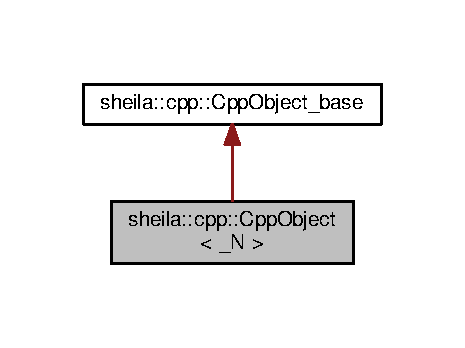
\includegraphics[width=223pt]{classsheila_1_1cpp_1_1CppObject__inherit__graph}
\end{center}
\end{figure}


Collaboration diagram for sheila\+:\+:cpp\+:\+:Cpp\+Object$<$ \+\_\+N $>$\+:
\nopagebreak
\begin{figure}[H]
\begin{center}
\leavevmode
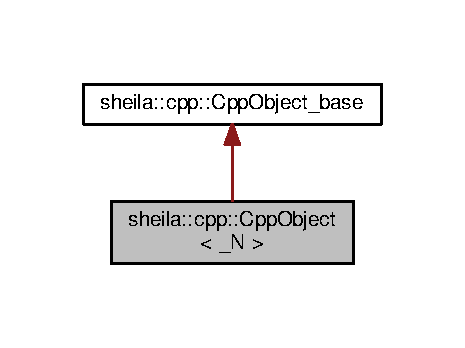
\includegraphics[width=223pt]{classsheila_1_1cpp_1_1CppObject__coll__graph}
\end{center}
\end{figure}
\subsection*{Public Member Functions}
\begin{DoxyCompactItemize}
\item 
\hyperlink{classsheila_1_1cpp_1_1CppObject_a16175f9d6ace3ea0bbb9e284984ed1fb}{Cpp\+Object} ()
\begin{DoxyCompactList}\small\item\em Creates a new abstract model of a C++ object. \end{DoxyCompactList}\item 
\hyperlink{classsheila_1_1cpp_1_1CppObject_a36c2625f6508c3886e0534c45fdff54f}{Cpp\+Object} (xml\+::\+Xml\+File $\ast$)
\begin{DoxyCompactList}\small\item\em Builds a new abstract model of a C++ object from an X\+ML file. \end{DoxyCompactList}\end{DoxyCompactItemize}


\subsection{Detailed Description}
\subsubsection*{template$<$class \+\_\+N$>$\\*
class sheila\+::cpp\+::\+Cpp\+Object$<$ \+\_\+\+N $>$}

An abstract model of a compilation object in C++. 

\begin{DoxyAuthor}{Author}
Flower\+Genius 
\end{DoxyAuthor}

\begin{DoxyTemplParams}{Template Parameters}
{\em \+\_\+N} & 1. {\ttfamily void} for typical usage; 2. {\ttfamily class} that this specialization will model.\\
\hline
\end{DoxyTemplParams}
This template class is very strange and possibly not clearly intuitive, thus this description may be too long to read, skip down to the end for a concise summary -\/ Flower\+Genius

Important Note\+: The strange nature of the class is a result of it\textquotesingle{}s intended usage, as this library is not meant for the understanding of a human developer, rather it is meant for the understanding of the Software Human Emulated Intelligence (on) Linux \mbox{[}a\mbox{]} a.\+k.\+a. {\ttfamily S\+H\+E\+I\+La}.

Introduction\+: For the purposes of this model, a C++ compilation object shall be defined as the combination of a single C++ source file and a definition of the user defined Header Files included from that source.

All header files included from those main header files shall not be {\itshape defined} by the object, rather they shall be referenced by the object. That is to say that when a {\ttfamily \hyperlink{classsheila_1_1cpp_1_1CppObject}{Cpp\+Object}} is represented in X\+ML, the X\+ML file contains only references to non-\/primary header files. Where the properties of them can be accessed through their pointer to their respective {\ttfamily Cpp\+Header} models such that modifications to those models modify them globally, rather than modifying a local copy of them.

An X\+ML representation of a {\ttfamily \hyperlink{classsheila_1_1cpp_1_1CppObject}{Cpp\+Object}} or one of it\textquotesingle{}s children must be a model of an entire valid X\+ML file.

Typical Usage (modeling a C++ compilation object) \+: {\ttfamily \hyperlink{classsheila_1_1cpp_1_1CppObject}{Cpp\+Object}$<${\itshape void} $>$} 

Adv. Usage (child models a C++ compilation object) \+: {\ttfamily \hyperlink{classsheila_1_1cpp_1_1CppObject}{Cpp\+Object}$<${\itshape \+\_\+N} $>$} where {\itshape \+\_\+N} is the class that the {\ttfamily \hyperlink{classsheila_1_1cpp_1_1CppObject}{Cpp\+Object}} is going to model.

TL;DR This class can be used as a typical class where the object that it represents is indicated by each unique instance of the class; OR it can be used as a template class where each unique specialization represents a compilation object. 

\subsection{Constructor \& Destructor Documentation}
\index{sheila\+::cpp\+::\+Cpp\+Object@{sheila\+::cpp\+::\+Cpp\+Object}!Cpp\+Object@{Cpp\+Object}}
\index{Cpp\+Object@{Cpp\+Object}!sheila\+::cpp\+::\+Cpp\+Object@{sheila\+::cpp\+::\+Cpp\+Object}}
\subsubsection[{\texorpdfstring{Cpp\+Object()}{CppObject()}}]{\setlength{\rightskip}{0pt plus 5cm}template$<$class \+\_\+N$>$ {\bf sheila\+::cpp\+::\+Cpp\+Object}$<$ \+\_\+N $>$\+::{\bf Cpp\+Object} (
\begin{DoxyParamCaption}
{}
\end{DoxyParamCaption}
)\hspace{0.3cm}{\ttfamily [inline]}}\hypertarget{classsheila_1_1cpp_1_1CppObject_a16175f9d6ace3ea0bbb9e284984ed1fb}{}\label{classsheila_1_1cpp_1_1CppObject_a16175f9d6ace3ea0bbb9e284984ed1fb}


Creates a new abstract model of a C++ object. 

\index{sheila\+::cpp\+::\+Cpp\+Object@{sheila\+::cpp\+::\+Cpp\+Object}!Cpp\+Object@{Cpp\+Object}}
\index{Cpp\+Object@{Cpp\+Object}!sheila\+::cpp\+::\+Cpp\+Object@{sheila\+::cpp\+::\+Cpp\+Object}}
\subsubsection[{\texorpdfstring{Cpp\+Object(xml\+::\+Xml\+File $\ast$)}{CppObject(xml::XmlFile *)}}]{\setlength{\rightskip}{0pt plus 5cm}template$<$class \+\_\+N$>$ {\bf sheila\+::cpp\+::\+Cpp\+Object}$<$ \+\_\+N $>$\+::{\bf Cpp\+Object} (
\begin{DoxyParamCaption}
\item[{xml\+::\+Xml\+File $\ast$}]{}
\end{DoxyParamCaption}
)}\hypertarget{classsheila_1_1cpp_1_1CppObject_a36c2625f6508c3886e0534c45fdff54f}{}\label{classsheila_1_1cpp_1_1CppObject_a36c2625f6508c3886e0534c45fdff54f}


Builds a new abstract model of a C++ object from an X\+ML file. 



The documentation for this class was generated from the following files\+:\begin{DoxyCompactItemize}
\item 
src/\+Cpp/\+Cpp\+Object/Cpp\+Object.\+h\item 
src/\+Cpp/\+Cpp\+Object/Cpp\+Object.\+cpp\end{DoxyCompactItemize}

\hypertarget{structsheila_1_1cpp_1_1CppObject__base}{}\section{sheila\+:\+:cpp\+:\+:Cpp\+Object\+\_\+base Struct Reference}
\label{structsheila_1_1cpp_1_1CppObject__base}\index{sheila\+::cpp\+::\+Cpp\+Object\+\_\+base@{sheila\+::cpp\+::\+Cpp\+Object\+\_\+base}}


The base for all of the specializations of {\ttfamily Cpp\+Class}.  




{\ttfamily \#include $<$Cpp\+Object.\+h$>$}



Inheritance diagram for sheila\+:\+:cpp\+:\+:Cpp\+Object\+\_\+base\+:
\nopagebreak
\begin{figure}[H]
\begin{center}
\leavevmode
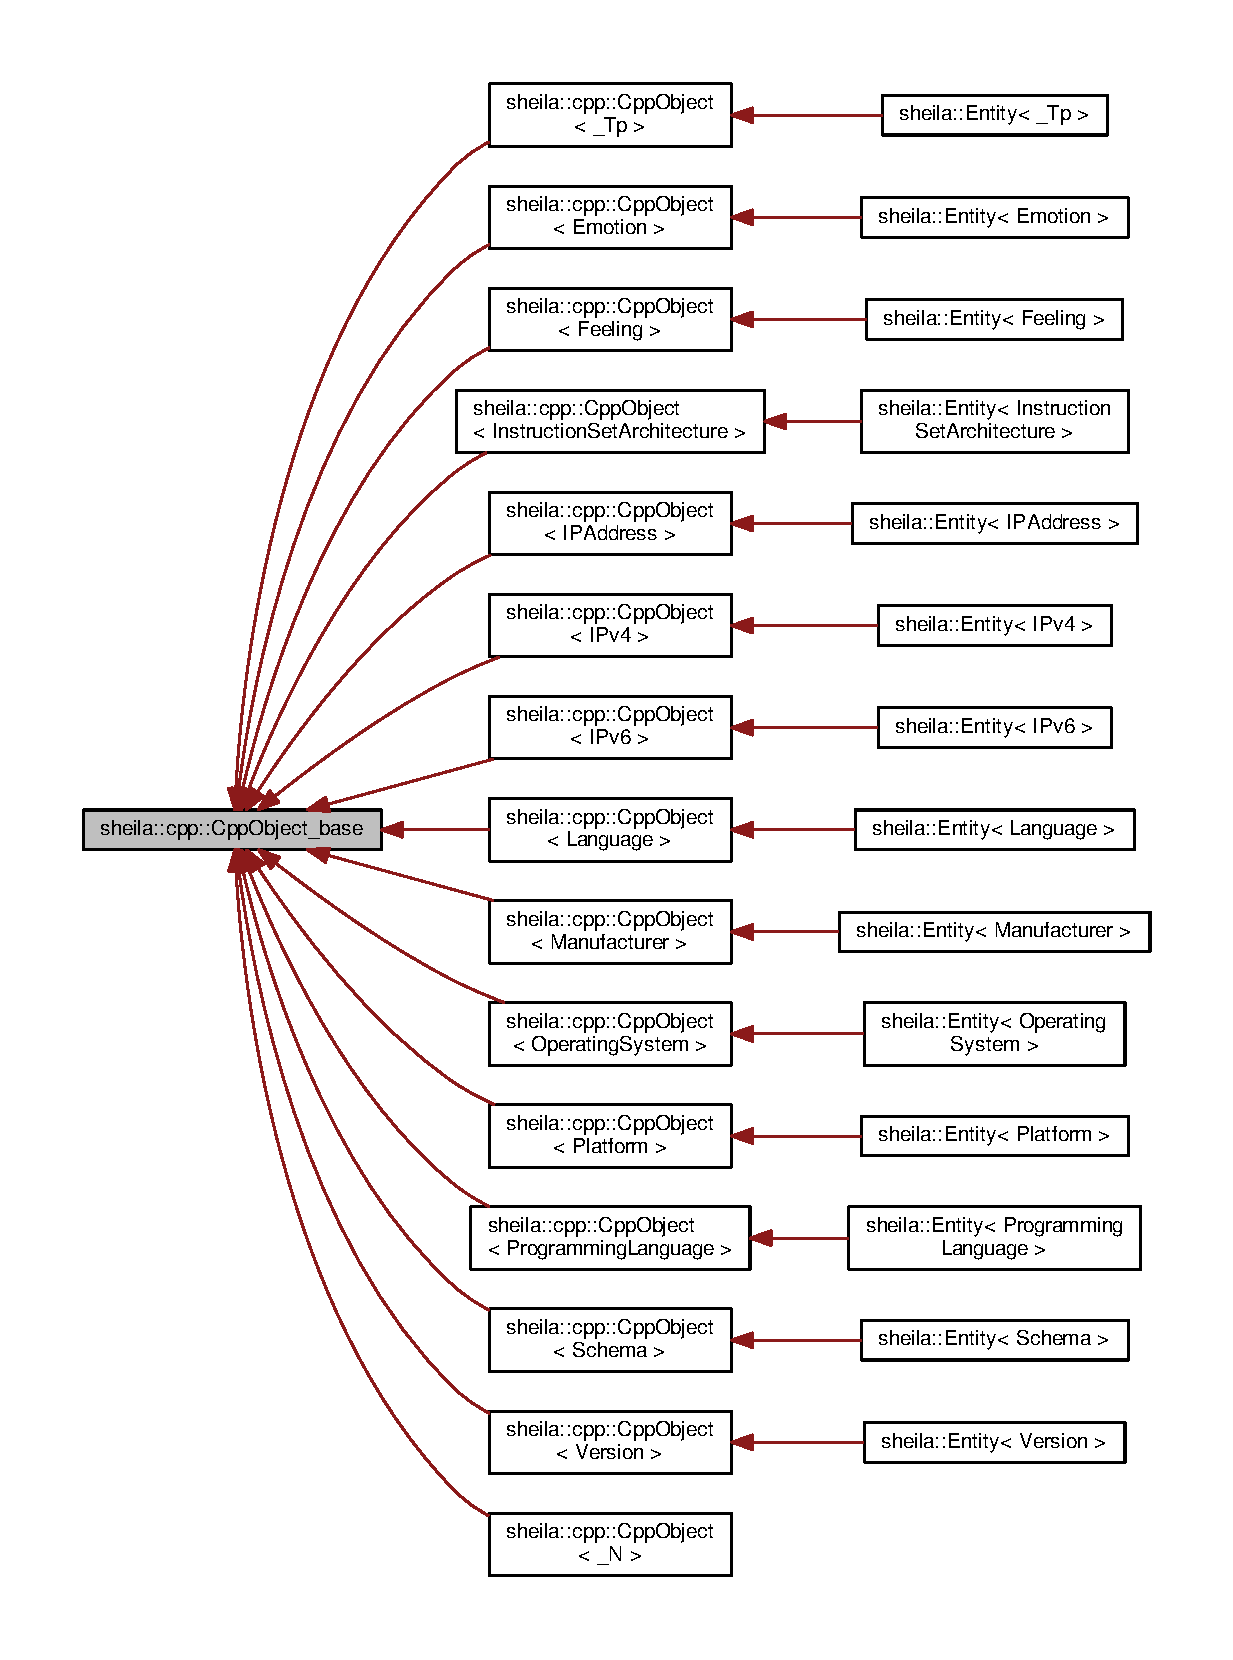
\includegraphics[width=350pt]{structsheila_1_1cpp_1_1CppObject__base__inherit__graph}
\end{center}
\end{figure}
\subsection*{Public Member Functions}
\begin{DoxyCompactItemize}
\item 
\hyperlink{structsheila_1_1cpp_1_1CppObject__base_ad2b023b8aa000845a49e3c09bb3ece64}{Cpp\+Object\+\_\+base} ()
\begin{DoxyCompactList}\small\item\em Default constructor for all specializations of {\ttfamily \hyperlink{classsheila_1_1cpp_1_1CppObject}{Cpp\+Object}}. \end{DoxyCompactList}\item 
virtual \hyperlink{structsheila_1_1cpp_1_1CppObject__base_aa5a1f3ffa146f2acfce90e1db2a9e5f9}{$\sim$\+Cpp\+Object\+\_\+base} ()
\begin{DoxyCompactList}\small\item\em Default destructor for all specializations of {\ttfamily \hyperlink{classsheila_1_1cpp_1_1CppObject}{Cpp\+Object}}. \end{DoxyCompactList}\end{DoxyCompactItemize}


\subsection{Detailed Description}
The base for all of the specializations of {\ttfamily Cpp\+Class}. 

\begin{DoxyAuthor}{Author}
Flower\+Genius
\end{DoxyAuthor}
This struct provides a base object for all of the specializations of {\ttfamily Cpp\+Class}. This struct is not meant to ever be used in it\textquotesingle{}s own right, rather it exists as a wrapper allowing any {\ttfamily \hyperlink{classsheila_1_1cpp_1_1CppObject}{Cpp\+Object}} types to be accessed, stored, and used iteratively by upcasting to this base. 

\subsection{Constructor \& Destructor Documentation}
\index{sheila\+::cpp\+::\+Cpp\+Object\+\_\+base@{sheila\+::cpp\+::\+Cpp\+Object\+\_\+base}!Cpp\+Object\+\_\+base@{Cpp\+Object\+\_\+base}}
\index{Cpp\+Object\+\_\+base@{Cpp\+Object\+\_\+base}!sheila\+::cpp\+::\+Cpp\+Object\+\_\+base@{sheila\+::cpp\+::\+Cpp\+Object\+\_\+base}}
\subsubsection[{\texorpdfstring{Cpp\+Object\+\_\+base()}{CppObject_base()}}]{\setlength{\rightskip}{0pt plus 5cm}sheila\+::cpp\+::\+Cpp\+Object\+\_\+base\+::\+Cpp\+Object\+\_\+base (
\begin{DoxyParamCaption}
{}
\end{DoxyParamCaption}
)\hspace{0.3cm}{\ttfamily [inline]}}\hypertarget{structsheila_1_1cpp_1_1CppObject__base_ad2b023b8aa000845a49e3c09bb3ece64}{}\label{structsheila_1_1cpp_1_1CppObject__base_ad2b023b8aa000845a49e3c09bb3ece64}


Default constructor for all specializations of {\ttfamily \hyperlink{classsheila_1_1cpp_1_1CppObject}{Cpp\+Object}}. 

\begin{DoxyAuthor}{Author}
Flower\+Genius
\end{DoxyAuthor}
This constructor should never be called excepting that it is called by a derived class as part of the derivation chain. \index{sheila\+::cpp\+::\+Cpp\+Object\+\_\+base@{sheila\+::cpp\+::\+Cpp\+Object\+\_\+base}!````~Cpp\+Object\+\_\+base@{$\sim$\+Cpp\+Object\+\_\+base}}
\index{````~Cpp\+Object\+\_\+base@{$\sim$\+Cpp\+Object\+\_\+base}!sheila\+::cpp\+::\+Cpp\+Object\+\_\+base@{sheila\+::cpp\+::\+Cpp\+Object\+\_\+base}}
\subsubsection[{\texorpdfstring{$\sim$\+Cpp\+Object\+\_\+base()}{~CppObject_base()}}]{\setlength{\rightskip}{0pt plus 5cm}virtual sheila\+::cpp\+::\+Cpp\+Object\+\_\+base\+::$\sim$\+Cpp\+Object\+\_\+base (
\begin{DoxyParamCaption}
{}
\end{DoxyParamCaption}
)\hspace{0.3cm}{\ttfamily [inline]}, {\ttfamily [virtual]}}\hypertarget{structsheila_1_1cpp_1_1CppObject__base_aa5a1f3ffa146f2acfce90e1db2a9e5f9}{}\label{structsheila_1_1cpp_1_1CppObject__base_aa5a1f3ffa146f2acfce90e1db2a9e5f9}


Default destructor for all specializations of {\ttfamily \hyperlink{classsheila_1_1cpp_1_1CppObject}{Cpp\+Object}}. 

\begin{DoxyAuthor}{Author}
Flower\+Genius
\end{DoxyAuthor}
This denstructor should never be called excepting that it is called by a derived class as part of the derivation chain. 

The documentation for this struct was generated from the following file\+:\begin{DoxyCompactItemize}
\item 
src/\+Cpp/\+Cpp\+Object/Cpp\+Object.\+h\end{DoxyCompactItemize}

\hypertarget{classsheila_1_1cpp_1_1CppPPDirective}{}\section{sheila\+:\+:cpp\+:\+:Cpp\+P\+P\+Directive$<$ \+\_\+\+Td $>$ Class Template Reference}
\label{classsheila_1_1cpp_1_1CppPPDirective}\index{sheila\+::cpp\+::\+Cpp\+P\+P\+Directive$<$ \+\_\+\+Td $>$@{sheila\+::cpp\+::\+Cpp\+P\+P\+Directive$<$ \+\_\+\+Td $>$}}


Generic \hyperlink{classsheila_1_1cpp_1_1CppPPDirective}{Cpp\+P\+P\+Directive} template class.  




{\ttfamily \#include $<$Cpp\+P\+P\+Directive.\+h$>$}



Inherits sheila\+::cpp\+::\+Cpp\+P\+P\+Directive\+\_\+base.

\subsection*{Public Member Functions}
\begin{DoxyCompactItemize}
\item 
std\+::string \hyperlink{classsheila_1_1cpp_1_1CppPPDirective_a5e99d12647c03da25f05fdb8f69ce207}{cpp\+\_\+str} ()
\begin{DoxyCompactList}\small\item\em Pure virtual member function promising the ability of derived types of {\ttfamily \hyperlink{classsheila_1_1cpp_1_1CppFeature}{Cpp\+Feature}} to be represented in C++ syntax. \end{DoxyCompactList}\item 
std\+::string \hyperlink{classsheila_1_1cpp_1_1CppPPDirective_ab3c20665d4ad7c66b9085175c084623e}{xml\+\_\+str} ()
\begin{DoxyCompactList}\small\item\em Pure virtual member function promising the ability of derived types of {\ttfamily \hyperlink{classsheila_1_1cpp_1_1CppFeature}{Cpp\+Feature}} to be represented in X\+ML syntax. \end{DoxyCompactList}\end{DoxyCompactItemize}


\subsection{Detailed Description}
\subsubsection*{template$<$Cpp\+P\+P\+Directive\+Type \+\_\+\+Td$>$\\*
class sheila\+::cpp\+::\+Cpp\+P\+P\+Directive$<$ \+\_\+\+Td $>$}

Generic \hyperlink{classsheila_1_1cpp_1_1CppPPDirective}{Cpp\+P\+P\+Directive} template class. 

\begin{DoxyAuthor}{Author}
Flower\+Genius 
\end{DoxyAuthor}

\begin{DoxyTemplParams}{Template Parameters}
{\em \+\_\+\+Td} & Type of C++ preprocessor directive.\\
\hline
\end{DoxyTemplParams}
Generic template for a C++ preprocessor directive, as there are a finite number of directives, templates are used with explicit specializations for each type of directive.

Author\textquotesingle{}s Note RE\+: The Generic \hyperlink{classsheila_1_1cpp_1_1CppPPDirective}{Cpp\+P\+P\+Directive} template class

While the generic template can be used and will almost always produce good code, it does not contribute to the code model and should be used sparingly.


\begin{DoxyItemize}
\item Flower\+Genius 
\end{DoxyItemize}

\subsection{Member Function Documentation}
\index{sheila\+::cpp\+::\+Cpp\+P\+P\+Directive@{sheila\+::cpp\+::\+Cpp\+P\+P\+Directive}!cpp\+\_\+str@{cpp\+\_\+str}}
\index{cpp\+\_\+str@{cpp\+\_\+str}!sheila\+::cpp\+::\+Cpp\+P\+P\+Directive@{sheila\+::cpp\+::\+Cpp\+P\+P\+Directive}}
\subsubsection[{\texorpdfstring{cpp\+\_\+str()}{cpp_str()}}]{\setlength{\rightskip}{0pt plus 5cm}template$<$Cpp\+P\+P\+Directive\+Type \+\_\+\+Td$>$ std\+::string {\bf sheila\+::cpp\+::\+Cpp\+P\+P\+Directive}$<$ \+\_\+\+Td $>$\+::cpp\+\_\+str (
\begin{DoxyParamCaption}
{}
\end{DoxyParamCaption}
)\hspace{0.3cm}{\ttfamily [virtual]}}\hypertarget{classsheila_1_1cpp_1_1CppPPDirective_a5e99d12647c03da25f05fdb8f69ce207}{}\label{classsheila_1_1cpp_1_1CppPPDirective_a5e99d12647c03da25f05fdb8f69ce207}


Pure virtual member function promising the ability of derived types of {\ttfamily \hyperlink{classsheila_1_1cpp_1_1CppFeature}{Cpp\+Feature}} to be represented in C++ syntax. 

\begin{DoxyAuthor}{Author}
Flower\+Genius 
\end{DoxyAuthor}
\begin{DoxyReturn}{Returns}
C++ string representing this feature in C++ syntax.
\end{DoxyReturn}
Since a {\ttfamily \hyperlink{classsheila_1_1cpp_1_1CppFeature}{Cpp\+Feature}} is a C++ lexical component, it must be able to be represented in valid and portable C++ syntax such that it can be inserted into a C++ file and form functioning code. 

Implements \hyperlink{classsheila_1_1cpp_1_1CppFeature_abe57540541227efa5c3e6ef2194276b9}{sheila\+::cpp\+::\+Cpp\+Feature}.

\index{sheila\+::cpp\+::\+Cpp\+P\+P\+Directive@{sheila\+::cpp\+::\+Cpp\+P\+P\+Directive}!xml\+\_\+str@{xml\+\_\+str}}
\index{xml\+\_\+str@{xml\+\_\+str}!sheila\+::cpp\+::\+Cpp\+P\+P\+Directive@{sheila\+::cpp\+::\+Cpp\+P\+P\+Directive}}
\subsubsection[{\texorpdfstring{xml\+\_\+str()}{xml_str()}}]{\setlength{\rightskip}{0pt plus 5cm}template$<$Cpp\+P\+P\+Directive\+Type \+\_\+\+Td$>$ std\+::string {\bf sheila\+::cpp\+::\+Cpp\+P\+P\+Directive}$<$ \+\_\+\+Td $>$\+::xml\+\_\+str (
\begin{DoxyParamCaption}
{}
\end{DoxyParamCaption}
)\hspace{0.3cm}{\ttfamily [virtual]}}\hypertarget{classsheila_1_1cpp_1_1CppPPDirective_ab3c20665d4ad7c66b9085175c084623e}{}\label{classsheila_1_1cpp_1_1CppPPDirective_ab3c20665d4ad7c66b9085175c084623e}


Pure virtual member function promising the ability of derived types of {\ttfamily \hyperlink{classsheila_1_1cpp_1_1CppFeature}{Cpp\+Feature}} to be represented in X\+ML syntax. 

\begin{DoxyAuthor}{Author}
Flower\+Genius 
\end{DoxyAuthor}
\begin{DoxyReturn}{Returns}
C++ string representing this feature in X\+ML syntax.
\end{DoxyReturn}
Since a {\ttfamily \hyperlink{classsheila_1_1cpp_1_1CppFeature}{Cpp\+Feature}} is a C++ lexical component, it can be represented using X\+ML.

In the C++ program structure model that is defined in the classes found in this library, any feature of C++ that can be represented in C++ syntax can also be represented in a strictly typed specialization of X\+ML that can be used to form a meta-\/level understanding of a C++ program and each of it\textquotesingle{}s individual components.

TL;DR Any feature of C++ can be represented as an X\+ML tag as well. 

Implements \hyperlink{classsheila_1_1cpp_1_1CppFeature_af32851fe8b1ce92bac4318605f0173db}{sheila\+::cpp\+::\+Cpp\+Feature}.



The documentation for this class was generated from the following files\+:\begin{DoxyCompactItemize}
\item 
src/\+Cpp/\+Cpp\+P\+P\+Directive/Cpp\+P\+P\+Directive.\+h\item 
src/\+Cpp/\+Cpp\+P\+P\+Directive/Cpp\+P\+P\+Directive.\+cpp\end{DoxyCompactItemize}

\hypertarget{classsheila_1_1cpp_1_1CppPPDirective_3_01CppPPDirectiveType_1_1DEFINE_01_4}{}\section{sheila\+:\+:cpp\+:\+:Cpp\+P\+P\+Directive$<$ Cpp\+P\+P\+Directive\+Type\+:\+:D\+E\+F\+I\+NE $>$ Class Template Reference}
\label{classsheila_1_1cpp_1_1CppPPDirective_3_01CppPPDirectiveType_1_1DEFINE_01_4}\index{sheila\+::cpp\+::\+Cpp\+P\+P\+Directive$<$ Cpp\+P\+P\+Directive\+Type\+::\+D\+E\+F\+I\+N\+E $>$@{sheila\+::cpp\+::\+Cpp\+P\+P\+Directive$<$ Cpp\+P\+P\+Directive\+Type\+::\+D\+E\+F\+I\+N\+E $>$}}


C++ Preprocessor directive specialization for a define directive.  




{\ttfamily \#include $<$Cpp\+P\+P\+Directive.\+h$>$}



Inherits sheila\+::cpp\+::\+Cpp\+P\+P\+Directive\+\_\+base.

\subsection*{Public Member Functions}
\begin{DoxyCompactItemize}
\item 
\hyperlink{classsheila_1_1cpp_1_1CppPPDirective_3_01CppPPDirectiveType_1_1DEFINE_01_4_a1511e565d049576911f8d04ce9628fad}{Cpp\+P\+P\+Directive} (\hyperlink{classsheila_1_1cpp_1_1CppFeature}{Cpp\+Feature} \&feat, std\+::string id, std\+::string statement, std\+::vector$<$ std\+::string $>$ args=\{\})
\begin{DoxyCompactList}\small\item\em Creates a model of a C++ define directive and a macro object. \end{DoxyCompactList}\item 
\hyperlink{classsheila_1_1cpp_1_1CppPPDirective_3_01CppPPDirectiveType_1_1DEFINE_01_4_a1b42adaa10edae5316be28b159485e35}{Cpp\+P\+P\+Directive} (\hyperlink{classsheila_1_1cpp_1_1CppFeature}{Cpp\+Feature} $\ast$feat, std\+::string id, std\+::string statement, std\+::vector$<$ std\+::string $>$ args=\{\})
\begin{DoxyCompactList}\small\item\em Creates a model of a C++ define directive and a macro object. \end{DoxyCompactList}\item 
std\+::string \hyperlink{classsheila_1_1cpp_1_1CppPPDirective_3_01CppPPDirectiveType_1_1DEFINE_01_4_a5fccebd381eeb594c6249eb2a0c70151}{cpp\+\_\+str} ()
\begin{DoxyCompactList}\small\item\em Pure virtual member function promising the ability of derived types of {\ttfamily \hyperlink{classsheila_1_1cpp_1_1CppFeature}{Cpp\+Feature}} to be represented in C++ syntax. \end{DoxyCompactList}\item 
std\+::string \hyperlink{classsheila_1_1cpp_1_1CppPPDirective_3_01CppPPDirectiveType_1_1DEFINE_01_4_ab46d249d848db43b0b0e4d28ea407bf3}{xml\+\_\+str} ()
\begin{DoxyCompactList}\small\item\em Pure virtual member function promising the ability of derived types of {\ttfamily \hyperlink{classsheila_1_1cpp_1_1CppFeature}{Cpp\+Feature}} to be represented in X\+ML syntax. \end{DoxyCompactList}\end{DoxyCompactItemize}


\subsection{Detailed Description}
\subsubsection*{template$<$$>$\\*
class sheila\+::cpp\+::\+Cpp\+P\+P\+Directive$<$ Cpp\+P\+P\+Directive\+Type\+::\+D\+E\+F\+I\+N\+E $>$}

C++ Preprocessor directive specialization for a define directive. 

\begin{DoxyAuthor}{Author}
Flower\+Genius
\end{DoxyAuthor}
An explicit specialization of the type D\+E\+F\+I\+NE that represents an abstract model of a C++ preprocessor define directive. 

\subsection{Constructor \& Destructor Documentation}
\index{sheila\+::cpp\+::\+Cpp\+P\+P\+Directive$<$ Cpp\+P\+P\+Directive\+Type\+::\+D\+E\+F\+I\+N\+E $>$@{sheila\+::cpp\+::\+Cpp\+P\+P\+Directive$<$ Cpp\+P\+P\+Directive\+Type\+::\+D\+E\+F\+I\+N\+E $>$}!Cpp\+P\+P\+Directive@{Cpp\+P\+P\+Directive}}
\index{Cpp\+P\+P\+Directive@{Cpp\+P\+P\+Directive}!sheila\+::cpp\+::\+Cpp\+P\+P\+Directive$<$ Cpp\+P\+P\+Directive\+Type\+::\+D\+E\+F\+I\+N\+E $>$@{sheila\+::cpp\+::\+Cpp\+P\+P\+Directive$<$ Cpp\+P\+P\+Directive\+Type\+::\+D\+E\+F\+I\+N\+E $>$}}
\subsubsection[{\texorpdfstring{Cpp\+P\+P\+Directive(\+Cpp\+Feature \&feat, std\+::string id, std\+::string statement, std\+::vector$<$ std\+::string $>$ args=\lcurly{}\rcurly{})}{CppPPDirective(CppFeature &feat, std::string id, std::string statement, std::vector< std::string > args=\{\})}}]{\setlength{\rightskip}{0pt plus 5cm}{\bf sheila\+::cpp\+::\+Cpp\+P\+P\+Directive}$<$ Cpp\+P\+P\+Directive\+Type\+::\+D\+E\+F\+I\+NE $>$\+::{\bf Cpp\+P\+P\+Directive} (
\begin{DoxyParamCaption}
\item[{{\bf Cpp\+Feature} \&}]{feat, }
\item[{std\+::string}]{id, }
\item[{std\+::string}]{statement, }
\item[{std\+::vector$<$ std\+::string $>$}]{args = {\ttfamily \{\}}}
\end{DoxyParamCaption}
)\hspace{0.3cm}{\ttfamily [inline]}}\hypertarget{classsheila_1_1cpp_1_1CppPPDirective_3_01CppPPDirectiveType_1_1DEFINE_01_4_a1511e565d049576911f8d04ce9628fad}{}\label{classsheila_1_1cpp_1_1CppPPDirective_3_01CppPPDirectiveType_1_1DEFINE_01_4_a1511e565d049576911f8d04ce9628fad}


Creates a model of a C++ define directive and a macro object. 

\begin{DoxyAuthor}{Author}
Flower\+Genius 
\end{DoxyAuthor}

\begin{DoxyParams}{Parameters}
{\em feat} & Reference to the C++ feature that comes immediately before this directive in the source code. \\
\hline
{\em id} & String that is a (typically) valid macro identifier. \\
\hline
{\em statement} & String that is a (typically) valid macro expression. \\
\hline
{\em args} & Vector of 0 or more strings for the macro arguments.\\
\hline
\end{DoxyParams}
This constructor generates an abstract model of a C++ define directive. It also creates a new macro object representing the macro that has been defined by the directive. \index{sheila\+::cpp\+::\+Cpp\+P\+P\+Directive$<$ Cpp\+P\+P\+Directive\+Type\+::\+D\+E\+F\+I\+N\+E $>$@{sheila\+::cpp\+::\+Cpp\+P\+P\+Directive$<$ Cpp\+P\+P\+Directive\+Type\+::\+D\+E\+F\+I\+N\+E $>$}!Cpp\+P\+P\+Directive@{Cpp\+P\+P\+Directive}}
\index{Cpp\+P\+P\+Directive@{Cpp\+P\+P\+Directive}!sheila\+::cpp\+::\+Cpp\+P\+P\+Directive$<$ Cpp\+P\+P\+Directive\+Type\+::\+D\+E\+F\+I\+N\+E $>$@{sheila\+::cpp\+::\+Cpp\+P\+P\+Directive$<$ Cpp\+P\+P\+Directive\+Type\+::\+D\+E\+F\+I\+N\+E $>$}}
\subsubsection[{\texorpdfstring{Cpp\+P\+P\+Directive(\+Cpp\+Feature $\ast$feat, std\+::string id, std\+::string statement, std\+::vector$<$ std\+::string $>$ args=\lcurly{}\rcurly{})}{CppPPDirective(CppFeature *feat, std::string id, std::string statement, std::vector< std::string > args=\{\})}}]{\setlength{\rightskip}{0pt plus 5cm}{\bf sheila\+::cpp\+::\+Cpp\+P\+P\+Directive}$<$ Cpp\+P\+P\+Directive\+Type\+::\+D\+E\+F\+I\+NE $>$\+::{\bf Cpp\+P\+P\+Directive} (
\begin{DoxyParamCaption}
\item[{{\bf Cpp\+Feature} $\ast$}]{feat, }
\item[{std\+::string}]{id, }
\item[{std\+::string}]{statement, }
\item[{std\+::vector$<$ std\+::string $>$}]{args = {\ttfamily \{\}}}
\end{DoxyParamCaption}
)\hspace{0.3cm}{\ttfamily [inline]}}\hypertarget{classsheila_1_1cpp_1_1CppPPDirective_3_01CppPPDirectiveType_1_1DEFINE_01_4_a1b42adaa10edae5316be28b159485e35}{}\label{classsheila_1_1cpp_1_1CppPPDirective_3_01CppPPDirectiveType_1_1DEFINE_01_4_a1b42adaa10edae5316be28b159485e35}


Creates a model of a C++ define directive and a macro object. 

\begin{DoxyAuthor}{Author}
Flower\+Genius 
\end{DoxyAuthor}

\begin{DoxyParams}{Parameters}
{\em feat} & Pointer to the C++ feature that comes immediately before this directive in the source code. \\
\hline
{\em id} & String that is a (typically) valid macro identifier. \\
\hline
{\em statement} & String that is a (typically) valid macro expression. \\
\hline
{\em args} & Vector of 0 or more strings for the macro arguments.\\
\hline
\end{DoxyParams}
This constructor generates an abstract model of a C++ define directive. It also creates a new macro object representing the macro that has been defined by the directive. 

\subsection{Member Function Documentation}
\index{sheila\+::cpp\+::\+Cpp\+P\+P\+Directive$<$ Cpp\+P\+P\+Directive\+Type\+::\+D\+E\+F\+I\+N\+E $>$@{sheila\+::cpp\+::\+Cpp\+P\+P\+Directive$<$ Cpp\+P\+P\+Directive\+Type\+::\+D\+E\+F\+I\+N\+E $>$}!cpp\+\_\+str@{cpp\+\_\+str}}
\index{cpp\+\_\+str@{cpp\+\_\+str}!sheila\+::cpp\+::\+Cpp\+P\+P\+Directive$<$ Cpp\+P\+P\+Directive\+Type\+::\+D\+E\+F\+I\+N\+E $>$@{sheila\+::cpp\+::\+Cpp\+P\+P\+Directive$<$ Cpp\+P\+P\+Directive\+Type\+::\+D\+E\+F\+I\+N\+E $>$}}
\subsubsection[{\texorpdfstring{cpp\+\_\+str()}{cpp_str()}}]{\setlength{\rightskip}{0pt plus 5cm}std\+::string {\bf sheila\+::cpp\+::\+Cpp\+P\+P\+Directive}$<$ Cpp\+P\+P\+Directive\+Type\+::\+D\+E\+F\+I\+NE $>$\+::cpp\+\_\+str (
\begin{DoxyParamCaption}
{}
\end{DoxyParamCaption}
)\hspace{0.3cm}{\ttfamily [inline]}, {\ttfamily [virtual]}}\hypertarget{classsheila_1_1cpp_1_1CppPPDirective_3_01CppPPDirectiveType_1_1DEFINE_01_4_a5fccebd381eeb594c6249eb2a0c70151}{}\label{classsheila_1_1cpp_1_1CppPPDirective_3_01CppPPDirectiveType_1_1DEFINE_01_4_a5fccebd381eeb594c6249eb2a0c70151}


Pure virtual member function promising the ability of derived types of {\ttfamily \hyperlink{classsheila_1_1cpp_1_1CppFeature}{Cpp\+Feature}} to be represented in C++ syntax. 

\begin{DoxyAuthor}{Author}
Flower\+Genius 
\end{DoxyAuthor}
\begin{DoxyReturn}{Returns}
C++ string representing this feature in C++ syntax.
\end{DoxyReturn}
Since a {\ttfamily \hyperlink{classsheila_1_1cpp_1_1CppFeature}{Cpp\+Feature}} is a C++ lexical component, it must be able to be represented in valid and portable C++ syntax such that it can be inserted into a C++ file and form functioning code. 

Implements \hyperlink{classsheila_1_1cpp_1_1CppFeature_abe57540541227efa5c3e6ef2194276b9}{sheila\+::cpp\+::\+Cpp\+Feature}.

\index{sheila\+::cpp\+::\+Cpp\+P\+P\+Directive$<$ Cpp\+P\+P\+Directive\+Type\+::\+D\+E\+F\+I\+N\+E $>$@{sheila\+::cpp\+::\+Cpp\+P\+P\+Directive$<$ Cpp\+P\+P\+Directive\+Type\+::\+D\+E\+F\+I\+N\+E $>$}!xml\+\_\+str@{xml\+\_\+str}}
\index{xml\+\_\+str@{xml\+\_\+str}!sheila\+::cpp\+::\+Cpp\+P\+P\+Directive$<$ Cpp\+P\+P\+Directive\+Type\+::\+D\+E\+F\+I\+N\+E $>$@{sheila\+::cpp\+::\+Cpp\+P\+P\+Directive$<$ Cpp\+P\+P\+Directive\+Type\+::\+D\+E\+F\+I\+N\+E $>$}}
\subsubsection[{\texorpdfstring{xml\+\_\+str()}{xml_str()}}]{\setlength{\rightskip}{0pt plus 5cm}std\+::string {\bf sheila\+::cpp\+::\+Cpp\+P\+P\+Directive}$<$ Cpp\+P\+P\+Directive\+Type\+::\+D\+E\+F\+I\+NE $>$\+::xml\+\_\+str (
\begin{DoxyParamCaption}
{}
\end{DoxyParamCaption}
)\hspace{0.3cm}{\ttfamily [inline]}, {\ttfamily [virtual]}}\hypertarget{classsheila_1_1cpp_1_1CppPPDirective_3_01CppPPDirectiveType_1_1DEFINE_01_4_ab46d249d848db43b0b0e4d28ea407bf3}{}\label{classsheila_1_1cpp_1_1CppPPDirective_3_01CppPPDirectiveType_1_1DEFINE_01_4_ab46d249d848db43b0b0e4d28ea407bf3}


Pure virtual member function promising the ability of derived types of {\ttfamily \hyperlink{classsheila_1_1cpp_1_1CppFeature}{Cpp\+Feature}} to be represented in X\+ML syntax. 

\begin{DoxyAuthor}{Author}
Flower\+Genius 
\end{DoxyAuthor}
\begin{DoxyReturn}{Returns}
C++ string representing this feature in X\+ML syntax.
\end{DoxyReturn}
Since a {\ttfamily \hyperlink{classsheila_1_1cpp_1_1CppFeature}{Cpp\+Feature}} is a C++ lexical component, it can be represented using X\+ML.

In the C++ program structure model that is defined in the classes found in this library, any feature of C++ that can be represented in C++ syntax can also be represented in a strictly typed specialization of X\+ML that can be used to form a meta-\/level understanding of a C++ program and each of it\textquotesingle{}s individual components.

TL;DR Any feature of C++ can be represented as an X\+ML tag as well. 

Implements \hyperlink{classsheila_1_1cpp_1_1CppFeature_af32851fe8b1ce92bac4318605f0173db}{sheila\+::cpp\+::\+Cpp\+Feature}.



The documentation for this class was generated from the following file\+:\begin{DoxyCompactItemize}
\item 
src/\+Cpp/\+Cpp\+P\+P\+Directive/Cpp\+P\+P\+Directive.\+h\end{DoxyCompactItemize}

\hypertarget{classsheila_1_1cpp_1_1CppPPDirective_3_01CppPPDirectiveType_1_1IFDEF_01_4}{}\section{sheila\+:\+:cpp\+:\+:Cpp\+P\+P\+Directive$<$ Cpp\+P\+P\+Directive\+Type\+:\+:I\+F\+D\+EF $>$ Class Template Reference}
\label{classsheila_1_1cpp_1_1CppPPDirective_3_01CppPPDirectiveType_1_1IFDEF_01_4}\index{sheila\+::cpp\+::\+Cpp\+P\+P\+Directive$<$ Cpp\+P\+P\+Directive\+Type\+::\+I\+F\+D\+E\+F $>$@{sheila\+::cpp\+::\+Cpp\+P\+P\+Directive$<$ Cpp\+P\+P\+Directive\+Type\+::\+I\+F\+D\+E\+F $>$}}


C++ Preprocessor directive specialization for an ifdef directive.  




{\ttfamily \#include $<$Cpp\+P\+P\+Directive.\+h$>$}



Inherits sheila\+::cpp\+::\+Cpp\+P\+P\+Directive\+\_\+base.

\subsection*{Public Member Functions}
\begin{DoxyCompactItemize}
\item 
\hyperlink{classsheila_1_1cpp_1_1CppPPDirective_3_01CppPPDirectiveType_1_1IFDEF_01_4_afe3dd5283d6163f3a391364f0843d040}{Cpp\+P\+P\+Directive} (Cpp\+Macro \&macro)
\begin{DoxyCompactList}\small\item\em Creates a model of a C++ ifdef directive. \end{DoxyCompactList}\item 
\hyperlink{classsheila_1_1cpp_1_1CppPPDirective_3_01CppPPDirectiveType_1_1IFDEF_01_4_a7a99bb6257f4addf5f92daca925dc2ae}{Cpp\+P\+P\+Directive} (Cpp\+Macro $\ast$macro)
\begin{DoxyCompactList}\small\item\em Creates a model of a C++ ifdef directive. \end{DoxyCompactList}\end{DoxyCompactItemize}


\subsection{Detailed Description}
\subsubsection*{template$<$$>$\\*
class sheila\+::cpp\+::\+Cpp\+P\+P\+Directive$<$ Cpp\+P\+P\+Directive\+Type\+::\+I\+F\+D\+E\+F $>$}

C++ Preprocessor directive specialization for an ifdef directive. 

\begin{DoxyAuthor}{Author}
Flower\+Genius
\end{DoxyAuthor}
An explicit specialization of the type I\+F\+D\+EF that represents an abstract model of a C++ preprocessor ifdef directive. 

\subsection{Constructor \& Destructor Documentation}
\index{sheila\+::cpp\+::\+Cpp\+P\+P\+Directive$<$ Cpp\+P\+P\+Directive\+Type\+::\+I\+F\+D\+E\+F $>$@{sheila\+::cpp\+::\+Cpp\+P\+P\+Directive$<$ Cpp\+P\+P\+Directive\+Type\+::\+I\+F\+D\+E\+F $>$}!Cpp\+P\+P\+Directive@{Cpp\+P\+P\+Directive}}
\index{Cpp\+P\+P\+Directive@{Cpp\+P\+P\+Directive}!sheila\+::cpp\+::\+Cpp\+P\+P\+Directive$<$ Cpp\+P\+P\+Directive\+Type\+::\+I\+F\+D\+E\+F $>$@{sheila\+::cpp\+::\+Cpp\+P\+P\+Directive$<$ Cpp\+P\+P\+Directive\+Type\+::\+I\+F\+D\+E\+F $>$}}
\subsubsection[{\texorpdfstring{Cpp\+P\+P\+Directive(\+Cpp\+Macro \&macro)}{CppPPDirective(CppMacro &macro)}}]{\setlength{\rightskip}{0pt plus 5cm}{\bf sheila\+::cpp\+::\+Cpp\+P\+P\+Directive}$<$ Cpp\+P\+P\+Directive\+Type\+::\+I\+F\+D\+EF $>$\+::{\bf Cpp\+P\+P\+Directive} (
\begin{DoxyParamCaption}
\item[{Cpp\+Macro \&}]{macro}
\end{DoxyParamCaption}
)\hspace{0.3cm}{\ttfamily [inline]}}\hypertarget{classsheila_1_1cpp_1_1CppPPDirective_3_01CppPPDirectiveType_1_1IFDEF_01_4_afe3dd5283d6163f3a391364f0843d040}{}\label{classsheila_1_1cpp_1_1CppPPDirective_3_01CppPPDirectiveType_1_1IFDEF_01_4_afe3dd5283d6163f3a391364f0843d040}


Creates a model of a C++ ifdef directive. 

\begin{DoxyAuthor}{Author}
Flower\+Genius 
\end{DoxyAuthor}

\begin{DoxyParams}{Parameters}
{\em macro} & Reference to the macro being tested for existence. \\
\hline
\end{DoxyParams}
\index{sheila\+::cpp\+::\+Cpp\+P\+P\+Directive$<$ Cpp\+P\+P\+Directive\+Type\+::\+I\+F\+D\+E\+F $>$@{sheila\+::cpp\+::\+Cpp\+P\+P\+Directive$<$ Cpp\+P\+P\+Directive\+Type\+::\+I\+F\+D\+E\+F $>$}!Cpp\+P\+P\+Directive@{Cpp\+P\+P\+Directive}}
\index{Cpp\+P\+P\+Directive@{Cpp\+P\+P\+Directive}!sheila\+::cpp\+::\+Cpp\+P\+P\+Directive$<$ Cpp\+P\+P\+Directive\+Type\+::\+I\+F\+D\+E\+F $>$@{sheila\+::cpp\+::\+Cpp\+P\+P\+Directive$<$ Cpp\+P\+P\+Directive\+Type\+::\+I\+F\+D\+E\+F $>$}}
\subsubsection[{\texorpdfstring{Cpp\+P\+P\+Directive(\+Cpp\+Macro $\ast$macro)}{CppPPDirective(CppMacro *macro)}}]{\setlength{\rightskip}{0pt plus 5cm}{\bf sheila\+::cpp\+::\+Cpp\+P\+P\+Directive}$<$ Cpp\+P\+P\+Directive\+Type\+::\+I\+F\+D\+EF $>$\+::{\bf Cpp\+P\+P\+Directive} (
\begin{DoxyParamCaption}
\item[{Cpp\+Macro $\ast$}]{macro}
\end{DoxyParamCaption}
)\hspace{0.3cm}{\ttfamily [inline]}}\hypertarget{classsheila_1_1cpp_1_1CppPPDirective_3_01CppPPDirectiveType_1_1IFDEF_01_4_a7a99bb6257f4addf5f92daca925dc2ae}{}\label{classsheila_1_1cpp_1_1CppPPDirective_3_01CppPPDirectiveType_1_1IFDEF_01_4_a7a99bb6257f4addf5f92daca925dc2ae}


Creates a model of a C++ ifdef directive. 

\begin{DoxyAuthor}{Author}
Flower\+Genius 
\end{DoxyAuthor}

\begin{DoxyParams}{Parameters}
{\em macro} & Pointer to the macro being tested for existence. \\
\hline
\end{DoxyParams}


The documentation for this class was generated from the following file\+:\begin{DoxyCompactItemize}
\item 
src/\+Cpp/\+Cpp\+P\+P\+Directive/Cpp\+P\+P\+Directive.\+h\end{DoxyCompactItemize}

\hypertarget{classsheila_1_1cpp_1_1CppPPDirective_3_01CppPPDirectiveType_1_1UNDEF_01_4}{}\section{sheila\+:\+:cpp\+:\+:Cpp\+P\+P\+Directive$<$ Cpp\+P\+P\+Directive\+Type\+:\+:U\+N\+D\+EF $>$ Class Template Reference}
\label{classsheila_1_1cpp_1_1CppPPDirective_3_01CppPPDirectiveType_1_1UNDEF_01_4}\index{sheila\+::cpp\+::\+Cpp\+P\+P\+Directive$<$ Cpp\+P\+P\+Directive\+Type\+::\+U\+N\+D\+E\+F $>$@{sheila\+::cpp\+::\+Cpp\+P\+P\+Directive$<$ Cpp\+P\+P\+Directive\+Type\+::\+U\+N\+D\+E\+F $>$}}


C++ Preprocessor directive specialization for an undef directive.  




{\ttfamily \#include $<$Cpp\+P\+P\+Directive.\+h$>$}



Inherits sheila\+::cpp\+::\+Cpp\+P\+P\+Directive\+\_\+base.

\subsection*{Public Member Functions}
\begin{DoxyCompactItemize}
\item 
\hyperlink{classsheila_1_1cpp_1_1CppPPDirective_3_01CppPPDirectiveType_1_1UNDEF_01_4_ae4dba686c72299618cb2811efc53da11}{Cpp\+P\+P\+Directive} (Cpp\+Macro \&macro)
\begin{DoxyCompactList}\small\item\em Creates a model of a C++ undef directive and marks a macro as undefined (destroying it\textquotesingle{}s contents). \end{DoxyCompactList}\item 
\hyperlink{classsheila_1_1cpp_1_1CppPPDirective_3_01CppPPDirectiveType_1_1UNDEF_01_4_af2ff6fd1bd46f18cbbd03e8e757f253c}{Cpp\+P\+P\+Directive} (Cpp\+Macro $\ast$macro)
\begin{DoxyCompactList}\small\item\em Creates a model of a C++ undef directive and marks a macro as undefined (destroying it\textquotesingle{}s contents). \end{DoxyCompactList}\end{DoxyCompactItemize}


\subsection{Detailed Description}
\subsubsection*{template$<$$>$\\*
class sheila\+::cpp\+::\+Cpp\+P\+P\+Directive$<$ Cpp\+P\+P\+Directive\+Type\+::\+U\+N\+D\+E\+F $>$}

C++ Preprocessor directive specialization for an undef directive. 

\begin{DoxyAuthor}{Author}
Flower\+Genius
\end{DoxyAuthor}
An explicit specialization of the type U\+N\+D\+EF that represents an abstract model of a C++ preprocessor undef directive. 

\subsection{Constructor \& Destructor Documentation}
\index{sheila\+::cpp\+::\+Cpp\+P\+P\+Directive$<$ Cpp\+P\+P\+Directive\+Type\+::\+U\+N\+D\+E\+F $>$@{sheila\+::cpp\+::\+Cpp\+P\+P\+Directive$<$ Cpp\+P\+P\+Directive\+Type\+::\+U\+N\+D\+E\+F $>$}!Cpp\+P\+P\+Directive@{Cpp\+P\+P\+Directive}}
\index{Cpp\+P\+P\+Directive@{Cpp\+P\+P\+Directive}!sheila\+::cpp\+::\+Cpp\+P\+P\+Directive$<$ Cpp\+P\+P\+Directive\+Type\+::\+U\+N\+D\+E\+F $>$@{sheila\+::cpp\+::\+Cpp\+P\+P\+Directive$<$ Cpp\+P\+P\+Directive\+Type\+::\+U\+N\+D\+E\+F $>$}}
\subsubsection[{\texorpdfstring{Cpp\+P\+P\+Directive(\+Cpp\+Macro \&macro)}{CppPPDirective(CppMacro &macro)}}]{\setlength{\rightskip}{0pt plus 5cm}{\bf sheila\+::cpp\+::\+Cpp\+P\+P\+Directive}$<$ Cpp\+P\+P\+Directive\+Type\+::\+U\+N\+D\+EF $>$\+::{\bf Cpp\+P\+P\+Directive} (
\begin{DoxyParamCaption}
\item[{Cpp\+Macro \&}]{macro}
\end{DoxyParamCaption}
)\hspace{0.3cm}{\ttfamily [inline]}}\hypertarget{classsheila_1_1cpp_1_1CppPPDirective_3_01CppPPDirectiveType_1_1UNDEF_01_4_ae4dba686c72299618cb2811efc53da11}{}\label{classsheila_1_1cpp_1_1CppPPDirective_3_01CppPPDirectiveType_1_1UNDEF_01_4_ae4dba686c72299618cb2811efc53da11}


Creates a model of a C++ undef directive and marks a macro as undefined (destroying it\textquotesingle{}s contents). 

\begin{DoxyAuthor}{Author}
Flower\+Genius 
\end{DoxyAuthor}

\begin{DoxyParams}{Parameters}
{\em macro} & Reference to the macro object to undefine. \\
\hline
\end{DoxyParams}
\index{sheila\+::cpp\+::\+Cpp\+P\+P\+Directive$<$ Cpp\+P\+P\+Directive\+Type\+::\+U\+N\+D\+E\+F $>$@{sheila\+::cpp\+::\+Cpp\+P\+P\+Directive$<$ Cpp\+P\+P\+Directive\+Type\+::\+U\+N\+D\+E\+F $>$}!Cpp\+P\+P\+Directive@{Cpp\+P\+P\+Directive}}
\index{Cpp\+P\+P\+Directive@{Cpp\+P\+P\+Directive}!sheila\+::cpp\+::\+Cpp\+P\+P\+Directive$<$ Cpp\+P\+P\+Directive\+Type\+::\+U\+N\+D\+E\+F $>$@{sheila\+::cpp\+::\+Cpp\+P\+P\+Directive$<$ Cpp\+P\+P\+Directive\+Type\+::\+U\+N\+D\+E\+F $>$}}
\subsubsection[{\texorpdfstring{Cpp\+P\+P\+Directive(\+Cpp\+Macro $\ast$macro)}{CppPPDirective(CppMacro *macro)}}]{\setlength{\rightskip}{0pt plus 5cm}{\bf sheila\+::cpp\+::\+Cpp\+P\+P\+Directive}$<$ Cpp\+P\+P\+Directive\+Type\+::\+U\+N\+D\+EF $>$\+::{\bf Cpp\+P\+P\+Directive} (
\begin{DoxyParamCaption}
\item[{Cpp\+Macro $\ast$}]{macro}
\end{DoxyParamCaption}
)\hspace{0.3cm}{\ttfamily [inline]}}\hypertarget{classsheila_1_1cpp_1_1CppPPDirective_3_01CppPPDirectiveType_1_1UNDEF_01_4_af2ff6fd1bd46f18cbbd03e8e757f253c}{}\label{classsheila_1_1cpp_1_1CppPPDirective_3_01CppPPDirectiveType_1_1UNDEF_01_4_af2ff6fd1bd46f18cbbd03e8e757f253c}


Creates a model of a C++ undef directive and marks a macro as undefined (destroying it\textquotesingle{}s contents). 

\begin{DoxyAuthor}{Author}
Flower\+Genius 
\end{DoxyAuthor}

\begin{DoxyParams}{Parameters}
{\em macro} & Pointer to the macro object to undefine. \\
\hline
\end{DoxyParams}


The documentation for this class was generated from the following file\+:\begin{DoxyCompactItemize}
\item 
src/\+Cpp/\+Cpp\+P\+P\+Directive/Cpp\+P\+P\+Directive.\+h\end{DoxyCompactItemize}

\hypertarget{classsheila_1_1Entity}{}\section{sheila\+:\+:Entity$<$ \+\_\+\+Tp $>$ Class Template Reference}
\label{classsheila_1_1Entity}\index{sheila\+::\+Entity$<$ \+\_\+\+Tp $>$@{sheila\+::\+Entity$<$ \+\_\+\+Tp $>$}}


Template class for an {\ttfamily \hyperlink{classsheila_1_1Entity}{Entity}} in the S\+H\+E\+I\+La structure model.  




{\ttfamily \#include $<$Entity.\+hpp$>$}



Inheritance diagram for sheila\+:\+:Entity$<$ \+\_\+\+Tp $>$\+:
\nopagebreak
\begin{figure}[H]
\begin{center}
\leavevmode
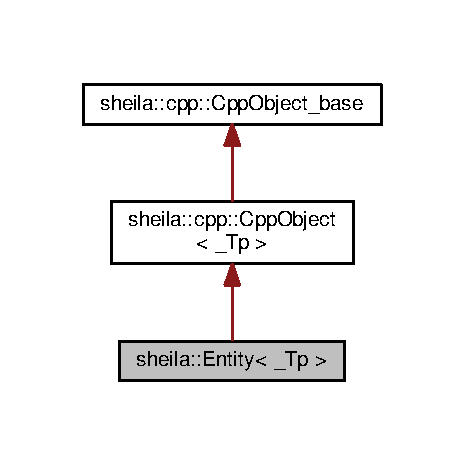
\includegraphics[width=223pt]{classsheila_1_1Entity__inherit__graph}
\end{center}
\end{figure}


Collaboration diagram for sheila\+:\+:Entity$<$ \+\_\+\+Tp $>$\+:
\nopagebreak
\begin{figure}[H]
\begin{center}
\leavevmode
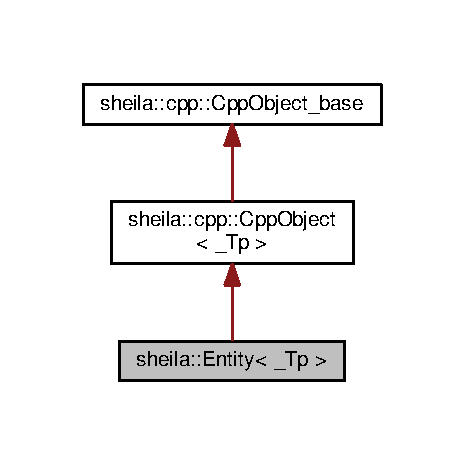
\includegraphics[width=223pt]{classsheila_1_1Entity__coll__graph}
\end{center}
\end{figure}
\subsection*{Public Member Functions}
\begin{DoxyCompactItemize}
\item 
\hyperlink{classsheila_1_1Entity_acd3c33a7c16f043198dc08980cc3e3a0}{Entity} ()
\begin{DoxyCompactList}\small\item\em Creates an {\ttfamily \hyperlink{classsheila_1_1Entity}{Entity}} for modifying the class of type {\itshape \+\_\+\+Tp}. \end{DoxyCompactList}\item 
virtual \hyperlink{classsheila_1_1Entity_ab658bb0db6c8dd6c35266f1416e55be1}{$\sim$\+Entity} ()
\begin{DoxyCompactList}\small\item\em Destroys an {\ttfamily \hyperlink{classsheila_1_1Entity}{Entity}} object. \end{DoxyCompactList}\end{DoxyCompactItemize}
\subsection*{Protected Member Functions}
\begin{DoxyCompactItemize}
\item 
virtual std\+::string \hyperlink{classsheila_1_1Entity_ae03819cad9837cc6620e345f4de4fb50}{\+\_\+\+E\+\_\+repr} ()
\begin{DoxyCompactList}\small\item\em Function returning a C++ string representing this instance. \end{DoxyCompactList}\item 
virtual void \hyperlink{classsheila_1_1Entity_aa19bb3e89281908d2a8c0ecc3b99005a}{\+\_\+\+E\+\_\+eval} (std\+::string repr)
\begin{DoxyCompactList}\small\item\em Function that re-\/creates an instance of $<$\+\_\+\+Tp$>$ from a C++ string. \end{DoxyCompactList}\end{DoxyCompactItemize}
\subsection*{Protected Attributes}
\begin{DoxyCompactItemize}
\item 
uintmax\+\_\+t \hyperlink{classsheila_1_1Entity_ad738ad7481e8575f577c821210ef95a5}{instance\+\_\+id}\hypertarget{classsheila_1_1Entity_ad738ad7481e8575f577c821210ef95a5}{}\label{classsheila_1_1Entity_ad738ad7481e8575f577c821210ef95a5}

\begin{DoxyCompactList}\small\item\em ID that is a unique unsigned integer within this object\textquotesingle{}s type. \end{DoxyCompactList}\item 
std\+::vector$<$ std\+::string $>$ \hyperlink{classsheila_1_1Entity_a781fe33d036a80709be80f34cd86a9b7}{instance\+\_\+name}\hypertarget{classsheila_1_1Entity_a781fe33d036a80709be80f34cd86a9b7}{}\label{classsheila_1_1Entity_a781fe33d036a80709be80f34cd86a9b7}

\begin{DoxyCompactList}\small\item\em List of all known aliases for the specific entity that this instance describes. \end{DoxyCompactList}\item 
std\+::vector$<$ std\+::string $>$ \hyperlink{classsheila_1_1Entity_a0befe31660d8a868d3ba435ede58b6e2}{instance\+\_\+desc}\hypertarget{classsheila_1_1Entity_a0befe31660d8a868d3ba435ede58b6e2}{}\label{classsheila_1_1Entity_a0befe31660d8a868d3ba435ede58b6e2}

\begin{DoxyCompactList}\small\item\em List of all known descriptions for the specific entity that this instance describes. \end{DoxyCompactList}\item 
std\+::vector$<$ std\+::string $>$ \hyperlink{classsheila_1_1Entity_a97a26ae1c5a05bbfc4d76e4f8beb67e5}{instance\+\_\+picture\+\_\+paths}\hypertarget{classsheila_1_1Entity_a97a26ae1c5a05bbfc4d76e4f8beb67e5}{}\label{classsheila_1_1Entity_a97a26ae1c5a05bbfc4d76e4f8beb67e5}

\begin{DoxyCompactList}\small\item\em List of paths to all known pictures of or containing the specific entity that this instance describes. \end{DoxyCompactList}\item 
std\+::vector$<$ std\+::string $>$ \hyperlink{classsheila_1_1Entity_a2285a01f1919bb408118991340b8865e}{instance\+\_\+video\+\_\+paths}\hypertarget{classsheila_1_1Entity_a2285a01f1919bb408118991340b8865e}{}\label{classsheila_1_1Entity_a2285a01f1919bb408118991340b8865e}

\begin{DoxyCompactList}\small\item\em List of paths to all known videos of or containing the specific entity that this instance describes. \end{DoxyCompactList}\item 
std\+::vector$<$ std\+::string $>$ \hyperlink{classsheila_1_1Entity_abcda4f7e450d957470a34cc9337e86bb}{instance\+\_\+sound\+\_\+paths}\hypertarget{classsheila_1_1Entity_abcda4f7e450d957470a34cc9337e86bb}{}\label{classsheila_1_1Entity_abcda4f7e450d957470a34cc9337e86bb}

\begin{DoxyCompactList}\small\item\em List of paths to all known audio files associated with the specific entity that this instance describes. \end{DoxyCompactList}\item 
std\+::vector$<$ std\+::string $>$ \hyperlink{classsheila_1_1Entity_a3dc9786a10315ffc78936cc403316531}{instance\+\_\+document\+\_\+paths}\hypertarget{classsheila_1_1Entity_a3dc9786a10315ffc78936cc403316531}{}\label{classsheila_1_1Entity_a3dc9786a10315ffc78936cc403316531}

\begin{DoxyCompactList}\small\item\em List of paths to all known document files associated with the specific entity that this instance describes. \end{DoxyCompactList}\item 
std\+::vector$<$ std\+::string $>$ \hyperlink{classsheila_1_1Entity_adaf94800aeaa342f516aaa403fdf5ca0}{instance\+\_\+program\+\_\+paths}\hypertarget{classsheila_1_1Entity_adaf94800aeaa342f516aaa403fdf5ca0}{}\label{classsheila_1_1Entity_adaf94800aeaa342f516aaa403fdf5ca0}

\begin{DoxyCompactList}\small\item\em List of paths to all known programs associated with the specific entity that this instance describes. \end{DoxyCompactList}\item 
std\+::vector$<$ long double $>$ \hyperlink{classsheila_1_1Entity_a66fd50c80c5ce05eddb8c21c77471dda}{instance\+\_\+emotion\+\_\+values}\hypertarget{classsheila_1_1Entity_a66fd50c80c5ce05eddb8c21c77471dda}{}\label{classsheila_1_1Entity_a66fd50c80c5ce05eddb8c21c77471dda}

\begin{DoxyCompactList}\small\item\em The emotional baggage that the (entity that this specific instance describes) carries. \end{DoxyCompactList}\item 
std\+::vector$<$ std\+::string $>$ \hyperlink{classsheila_1_1Entity_a4949571bc1564f6d2c1796953efda688}{instance\+\_\+cv\+\_\+filters}\hypertarget{classsheila_1_1Entity_a4949571bc1564f6d2c1796953efda688}{}\label{classsheila_1_1Entity_a4949571bc1564f6d2c1796953efda688}

\begin{DoxyCompactList}\small\item\em List of paths to all known schemas for identifying the entity that this specific instance describes. \end{DoxyCompactList}\end{DoxyCompactItemize}


\subsection{Detailed Description}
\subsubsection*{template$<$class \+\_\+\+Tp$>$\\*
class sheila\+::\+Entity$<$ \+\_\+\+Tp $>$}

Template class for an {\ttfamily \hyperlink{classsheila_1_1Entity}{Entity}} in the S\+H\+E\+I\+La structure model. 

\begin{DoxyAuthor}{Author}
Flower\+Genius 
\end{DoxyAuthor}

\begin{DoxyTemplParams}{Template Parameters}
{\em \+\_\+\+Tp} & The class that this {\ttfamily \hyperlink{classsheila_1_1Entity}{Entity}} will represent.\\
\hline
\end{DoxyTemplParams}
An {\ttfamily \hyperlink{classsheila_1_1Entity}{Entity}} is a special data type, it represents the pair of files required to build the class of the same name and it\textquotesingle{}s variants. 

\subsection{Constructor \& Destructor Documentation}
\index{sheila\+::\+Entity@{sheila\+::\+Entity}!Entity@{Entity}}
\index{Entity@{Entity}!sheila\+::\+Entity@{sheila\+::\+Entity}}
\subsubsection[{\texorpdfstring{Entity()}{Entity()}}]{\setlength{\rightskip}{0pt plus 5cm}template$<$class \+\_\+\+Tp$>$ {\bf sheila\+::\+Entity}$<$ \+\_\+\+Tp $>$\+::{\bf Entity} (
\begin{DoxyParamCaption}
{}
\end{DoxyParamCaption}
)\hspace{0.3cm}{\ttfamily [inline]}}\hypertarget{classsheila_1_1Entity_acd3c33a7c16f043198dc08980cc3e3a0}{}\label{classsheila_1_1Entity_acd3c33a7c16f043198dc08980cc3e3a0}


Creates an {\ttfamily \hyperlink{classsheila_1_1Entity}{Entity}} for modifying the class of type {\itshape \+\_\+\+Tp}. 

\begin{DoxyAuthor}{Author}
Flower\+Genius 
\end{DoxyAuthor}
\index{sheila\+::\+Entity@{sheila\+::\+Entity}!````~Entity@{$\sim$\+Entity}}
\index{````~Entity@{$\sim$\+Entity}!sheila\+::\+Entity@{sheila\+::\+Entity}}
\subsubsection[{\texorpdfstring{$\sim$\+Entity()}{~Entity()}}]{\setlength{\rightskip}{0pt plus 5cm}template$<$class \+\_\+\+Tp$>$ virtual {\bf sheila\+::\+Entity}$<$ \+\_\+\+Tp $>$\+::$\sim${\bf Entity} (
\begin{DoxyParamCaption}
{}
\end{DoxyParamCaption}
)\hspace{0.3cm}{\ttfamily [inline]}, {\ttfamily [virtual]}}\hypertarget{classsheila_1_1Entity_ab658bb0db6c8dd6c35266f1416e55be1}{}\label{classsheila_1_1Entity_ab658bb0db6c8dd6c35266f1416e55be1}


Destroys an {\ttfamily \hyperlink{classsheila_1_1Entity}{Entity}} object. 

\begin{DoxyAuthor}{Author}
Flower\+Genius 
\end{DoxyAuthor}


\subsection{Member Function Documentation}
\index{sheila\+::\+Entity@{sheila\+::\+Entity}!\+\_\+\+E\+\_\+eval@{\+\_\+\+E\+\_\+eval}}
\index{\+\_\+\+E\+\_\+eval@{\+\_\+\+E\+\_\+eval}!sheila\+::\+Entity@{sheila\+::\+Entity}}
\subsubsection[{\texorpdfstring{\+\_\+\+E\+\_\+eval(std\+::string repr)}{_E_eval(std::string repr)}}]{\setlength{\rightskip}{0pt plus 5cm}template$<$class \+\_\+\+Tp$>$ virtual void {\bf sheila\+::\+Entity}$<$ \+\_\+\+Tp $>$\+::\+\_\+\+E\+\_\+eval (
\begin{DoxyParamCaption}
\item[{std\+::string}]{repr}
\end{DoxyParamCaption}
)\hspace{0.3cm}{\ttfamily [inline]}, {\ttfamily [protected]}, {\ttfamily [virtual]}}\hypertarget{classsheila_1_1Entity_aa19bb3e89281908d2a8c0ecc3b99005a}{}\label{classsheila_1_1Entity_aa19bb3e89281908d2a8c0ecc3b99005a}


Function that re-\/creates an instance of $<$\+\_\+\+Tp$>$ from a C++ string. 

\begin{DoxyAuthor}{Author}
Flower\+Genius 
\end{DoxyAuthor}

\begin{DoxyParams}{Parameters}
{\em repr} & A C++ string that represents an instance of {\ttfamily Entity$<$\+\_\+\+Tp$>$} \\
\hline
\end{DoxyParams}
\index{sheila\+::\+Entity@{sheila\+::\+Entity}!\+\_\+\+E\+\_\+repr@{\+\_\+\+E\+\_\+repr}}
\index{\+\_\+\+E\+\_\+repr@{\+\_\+\+E\+\_\+repr}!sheila\+::\+Entity@{sheila\+::\+Entity}}
\subsubsection[{\texorpdfstring{\+\_\+\+E\+\_\+repr()}{_E_repr()}}]{\setlength{\rightskip}{0pt plus 5cm}template$<$class \+\_\+\+Tp$>$ virtual std\+::string {\bf sheila\+::\+Entity}$<$ \+\_\+\+Tp $>$\+::\+\_\+\+E\+\_\+repr (
\begin{DoxyParamCaption}
{}
\end{DoxyParamCaption}
)\hspace{0.3cm}{\ttfamily [inline]}, {\ttfamily [protected]}, {\ttfamily [virtual]}}\hypertarget{classsheila_1_1Entity_ae03819cad9837cc6620e345f4de4fb50}{}\label{classsheila_1_1Entity_ae03819cad9837cc6620e345f4de4fb50}


Function returning a C++ string representing this instance. 

\begin{DoxyAuthor}{Author}
Flower\+Genius 
\end{DoxyAuthor}
\begin{DoxyReturn}{Returns}
A strictly formatted C++ string.
\end{DoxyReturn}
Returns a C++ string that can be parsed by {\ttfamily \hyperlink{classsheila_1_1Entity_aa19bb3e89281908d2a8c0ecc3b99005a}{\+\_\+\+E\+\_\+eval()}} to re-\/create an exact copy of this specific instance. 

The documentation for this class was generated from the following files\+:\begin{DoxyCompactItemize}
\item 
src/\+Entity/Entity.\+hpp\item 
src/\+Entity/Entity.\+cpp\end{DoxyCompactItemize}

%--- End generated contents ---

% Index
\backmatter
\newpage
\phantomsection
\clearemptydoublepage
\addcontentsline{toc}{chapter}{Index}
\printindex

\end{document}
